%%%%%%%%%%%%%%%%%%%%%%%%%%%%%%%%%%%%%%%%%%%%%%%%%%%%%%%%%%%%%%%%%%%%%%%%%%%%%%%%%%%%%%%%%%%%%%%%%%%
% Chapter 2 -> Background
% Author: Mingbo Cheng
%%%%%%%%%%%%%%%%%%%%%%%%%%%%%%%%%%%%%%%%%%%%%%%%%%%%%%%%%%%%%%%%%%%%%%%%%%%%%%%%%%%%%%%%%%%%%%%%%%%
%\addbibresource{~/MEGA/MEGAsync/phd/thesis_Cheng/preamble/thesis.bib}
%\addbibresource{/home/mingbo/MEGAsync/phd/thesis_Cheng/preamble/thesis.bib}
\chapter{Background}
\label{cha:background}
\graphicspath{{chapter2/figs/}}

In this chapter, we provide a comprehensive overview of the background knowledge necessary for understanding the thesis, encompassing both biological and computational aspects. We begin by delving into molecular biology involving DNA organization, chromatin accessibility, and gene regulation~(Section 2.1). Next, we explore the advancements in single-cell sequencing technologies, covering single-cell transcriptome profiling, and open chromatin measurements in single cells. This section also encompasses sequencing protocols capable of simultaneously measuring multiple types of features, known as multimodal sequencing~(Section 2.2). Following that, we introduce computational approaches for analyzing various single-cell technology assays including single-cell RNA-seq analysis, single-cell ATAC-seq analysis, and single-cell surface protein analysis~(Section 2.3). Subsequently, we present the computational workflow for multimodal analysis. Following that, we outline two main problems that need to be addressed in single-cell multimodal analysis. The first problem is multimodal integration. For this, we first discuss the challenges associated with the task. We then introduce the current state-of-the-art methods for multimodal integration, aligning with our objective to address the issues. The second problem is trajectory inference for multimodal data. Similarly, we first present the challenge of trajectory inference. Next, we introduce the current state-of-the-art methods for trajectory inference, aligning with our goals for solving the trajectory inference issues in our method~(Section 2.4). Finally, we conclude the chapter with a final discussion on the background~(Section 2.5).


\section{DNA Organization, chromatin accessibility and gene regulation}
\label{background:DNA_Chromatin_Regulation}
In the symphony of life, the function of DNA organization, chromatin accessibility, and gene regulation orchestrates a harmonious dance that dictates the fate and functioning of every living organism. This dance is involved in the process in the central dogma of molecular biology~\citep{crick1970central} which describes the process by which genetic information is transferred from DNA to RNA and eventually translated to protein~(\fref{fig:central_dogma}). We start this section by first introducing DNA organization. Next, we talk about gene regulation followed by the introduction of chromatin accessibility.

\begin{figure}[!ht]
	\centering
	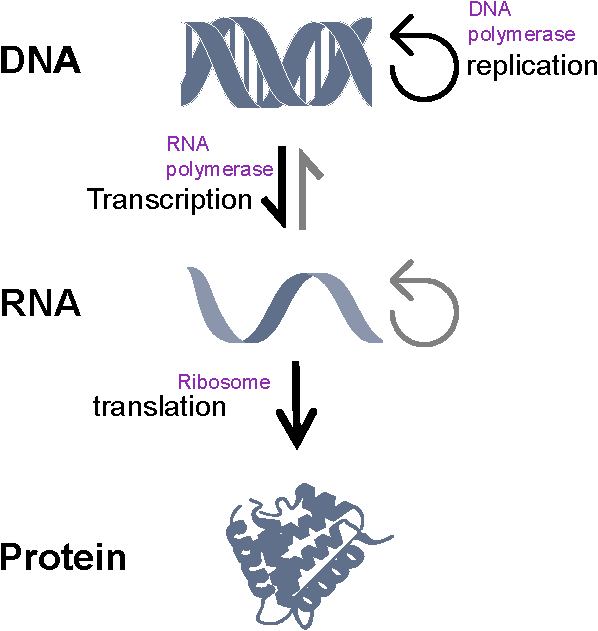
\includegraphics[width=0.65\textwidth]{central_dogma/fig}
	\vspace{0.1cm}
	\caption[central dogma.]{Central dogma of molecular biology including DNA replication, transcription and RNA translation.}
	\label{fig:central_dogma}
\end{figure}

Deoxyribonucleic Acid, or DNA is the genetic blueprint of life, containing the instructions for the development and functioning of living organisms. It is a long, double-stranded helical structure composed of four nucleotide building blocks: adenine (A), thymine (T), cytosine (C), and guanine (G). The sequence of these nucleotides forms the genetic code, encoding instructions for the development, functioning, and maintenance of all living organisms. DNA is organized into structures called chromosomes, which are located in the cell nucleus.



Gene regulation refers to the mechanisms that control the expression of genes. While an organism's DNA carries the instructions for a vast array of biological processes, not all genes are active all the time. Gene regulation allows cells to turn genes on or off, and to fine-tune their activity. This regulation is achieved through the interaction of regulatory proteins, transcription factors, and other molecules that bind to specific DNA sequences, influencing the initiation or inhibition of transcription. The transcribed RNAs next undergo a crucial process known as splicing, wherein a single pre-mRNA can give rise to various mRNAs. Following this, the resulting mRNAs are translated into proteins, and these proteins may undergo multiple post-translational modifications that can impact their activity. These modifications include ubiquitylation, methylation, phosphorylation, or acetylation~\citep{wang2014protein} (\fref{fig:central_dogma}).

%Epigenetic modifications, such as DNA methylation and histone modification, also play a crucial role in gene regulation by modifying the accessibility of DNA.

\begin{figure}[!ht]
	\centering
	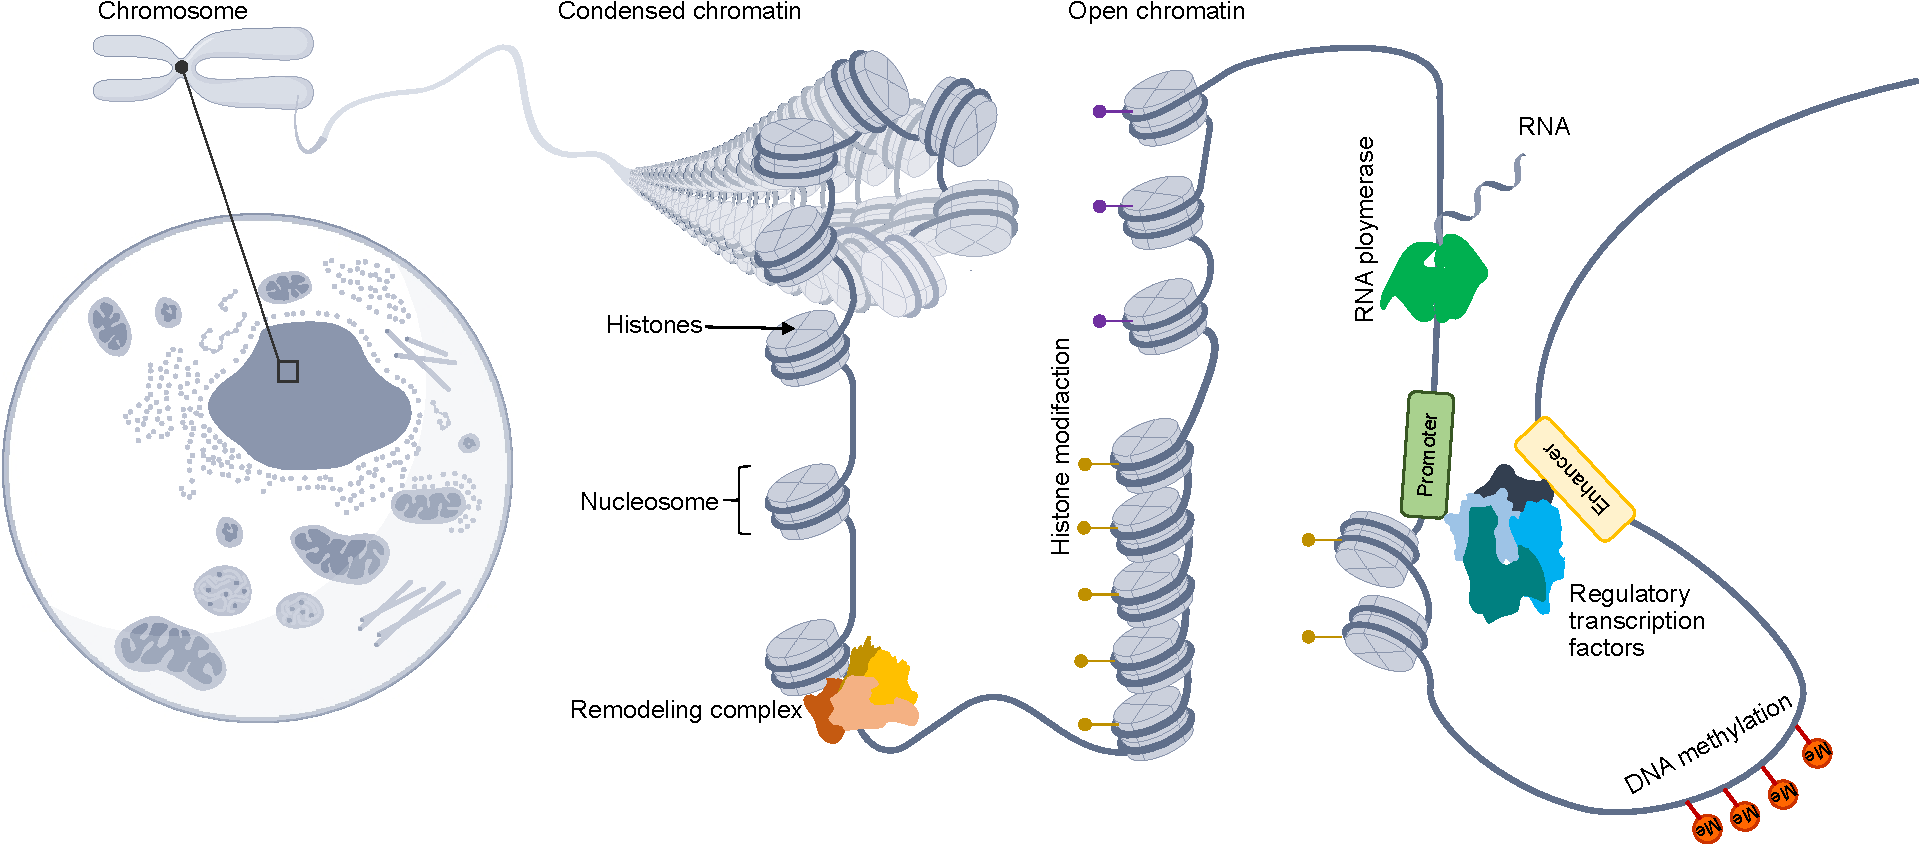
\includegraphics[width=0.95\textwidth]{chromatin_organization/fig}
	\vspace{0.1cm}
	\caption[DNA organization] {DNA is directed, controlled, and regulated by epithatic factors which surround and scaffold DNA in order to orchestrate the cellular mechanisms of life. The epigenome is the collection of DNA, RNA, proteins, and their chemical modifications that alter gene expression without changing the genetic code. Epigenetic machinery modifies the accessibility of regions in DNA by adding marks to the tails of histones, creating epigenetic patterns of chromatin modifications. The addition of an acetyl group to a histone tail changes the electrochemical charge of the histone, causing it to relax and release the DNA. This makes the DNA in that region more accessible to transcription machinery and allows that gene to be expressed. Placing a methyl group on histone tails can either increase or decrease the pattern of gene expression, depending on where the mark is placed. Additionally, placing a methyl group directly onto the DNA results in the permanent shutdown of that genetic region. \emph{Source:~\cite{heumos2023best}}~(modified to fit thesis format and/or clarify key points)}
	\label{fig:chromatin_organization}
\end{figure}


Chromatin is the complex of DNA and proteins found in the nucleus of a cell. Chromatin accessibility is a crucial molecular concept that describes the degree to which DNA is available or accessible for cellular processes, particularly gene expression. It can exist in two states: open and condensed. Open chromatin refers to the relaxed, accessible state where DNA is available for transcription and gene expression. In this state, the DNA is not tightly wound around histone proteins, allowing regulatory proteins and RNA polymerase to easily access specific DNA sequences, facilitating the transcription of genes into RNA. Open chromatin is associated with active gene expression and is influenced by various factors, including epigenetic modifications such as acetylation and methylation. Conversely, in a "closed" or condensed chromatin state, the DNA is tightly wound around histone proteins, making it less accessible. This state inhibits the binding of transcriptional machinery, leading to reduced or suppressed gene expression. Closed chromatin is associated with inactive or silenced genes (\fref{fig:chromatin_organization}).




\section{Single cell sequencing technology}
\label{background:profiling_singlecell}
The invention of a series of rapidly evolving Next Generation Sequencing~(NGS) technologies revolutionarily facilitates the study of heterogeneous biological processes with high throughput, shorter time and lower cost~\citep{svensson2018exponential}. NGS enables researchers to perform profiling of epigenomes, transcriptomes and proteomes and the development of single-cell sequencing technology further facilitates the study of heterogeneity at single-cell resolution. In this section, we will briefly introduce single-cell sequencing technology, single-cell RNA sequencing, single-cell ATAC sequencing and single-cell protein sequencing.

To begin, let's establish clear definitions for Genome, Epigenome, Transcriptome, and Proteome. Genome is the complete set of DNA, which holds all the genetic information of an organism~\citep{hubbard2002genome}, Epigenome is the complete set of reversible chemical changes to the DNA and histone proteins of an organism~\citep{bernstein2007epigenome}, Transcriptome is the complete set of RNA molecules in a cell or a collection of cells~\citep{haoudi2006proteome}, Proteome is the complete set of proteins expressed in a cell, tissue, or organism~\citep{wang2009transcriptome}. The term “-omics” refer to the exploration of corresponding omic data. Genomics specifically focuses on the investigation of an organism's genome. Likewise, Epigenomics, Transcriptomics, and Proteomics encompass the study of epigenomes, transcriptomes, and proteomes, respectively.


\subsection{Transcriptomics profiling with scRNA-seq}
\label{background:sec1:scRNA}

Single-cell RNA sequencing~(scRNA-seq)~\citep{singlecellsequencing2014, singlecellsequencing2015} has emerged as a powerful tool that allows the study of gene expression at the individual cell level, providing insights into the heterogeneity and dynamics of cellular responses in various biological contexts. In contrast to traditional bulk RNA-seq, which averages gene expression across millions of cells, scRNA-seq enables the investigation of transcriptomic profiles within specific cell types, offering a more detailed understanding of cellular behaviors during development or in response to perturbations.

\begin{figure}[!ht]
	\centering
	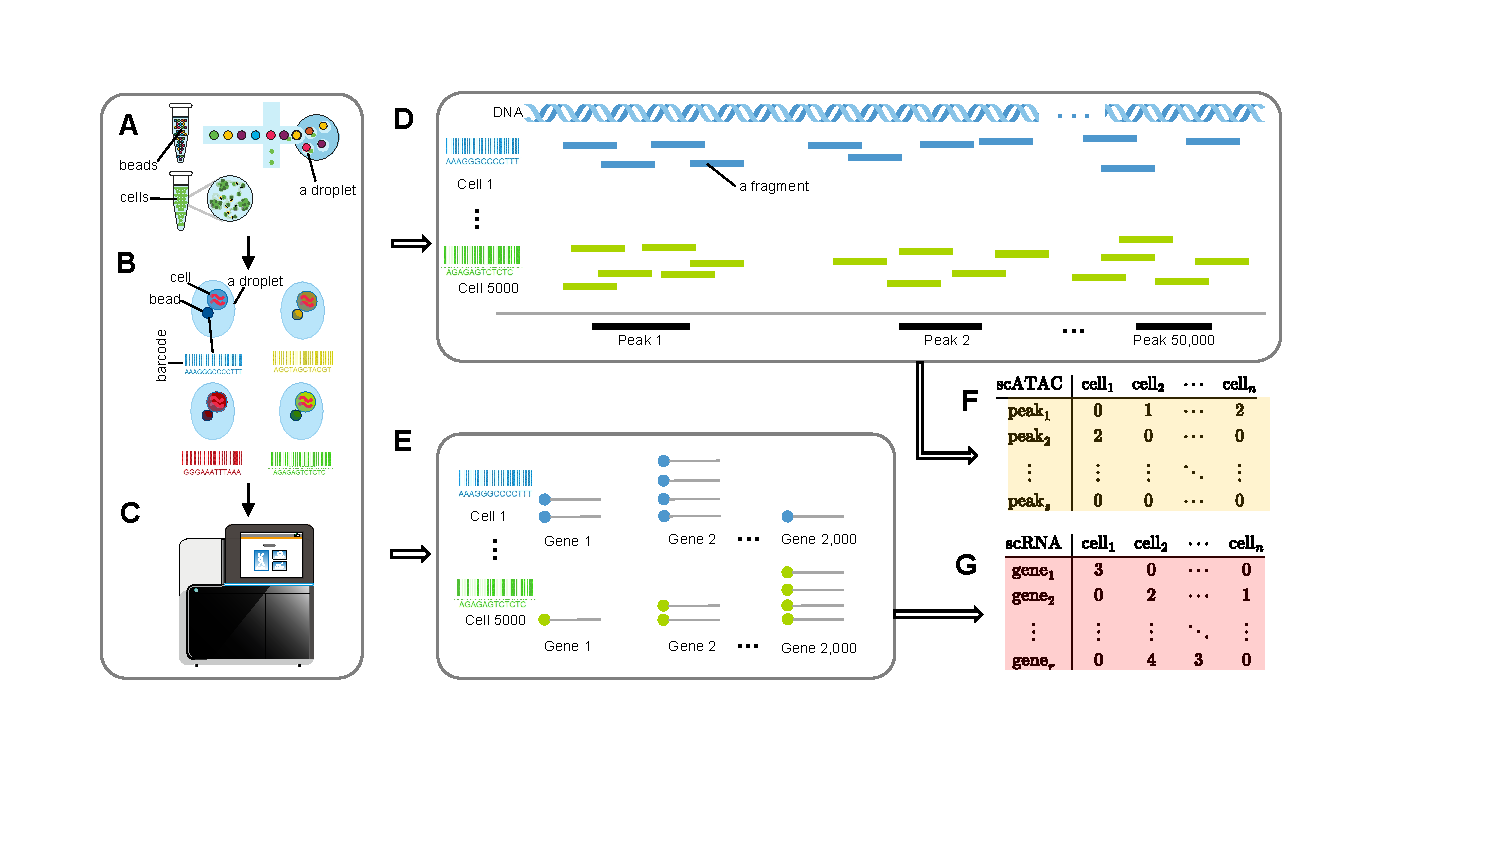
\includegraphics[width=0.95\textwidth]{Sequencing/fig}
	\vspace{0.1cm}
	\caption[Droplet-based simultaneous single-cell sequencing of transcriptome and epigenome.]{\textbf{Droplet-based simultaneous single-cell sequencing of transcriptome and epigenome.} \textbf{A)} The top left depicts Gel beads with a barcode fragment each. The bottom left shows a single nuclei suspension with single nuclei RNA and single nuclei ATAC-seq fragments. On the right, there's a Gel bead barcode that will attach to a single cell, forming a droplet. \textbf{B)} Four droplets are displayed, each containing a bead with a barcode fragment and a single cell. Barcodes uniquely identify individual cells. \textbf{C)} Droplets with single cells are isolated for sequencing, generating single cell RNA-seq and single ATAC-seq libraries. \textbf{D)} Sequencing outputs single cell ATAC-seq fragments, and alignment to reference DNA reveals fragment distributions with peaks at specific DNA positions. \textbf{E)} Sequencing also outputs single-cell RNA reads, identifying specific genes with each gene's molecular count tagged with a Unique Molecular Identifier (UMI). \textbf{F)} Counting the peaks in each single cell (cell barcode) constructs a peak-by-cell count matrix for scATAC-seq data. \textbf{G)} Counting the UMIs of each single cell (cell barcode) constructs a gene-by-cell count matrix for scRNA-seq data.}
	\label{fig:scRNA_scATAC_to_count_matrix}
\end{figure}

Single-cell RNA sequencing~(scRNA-seq) was introduced in 2009~\citep{tang2009mrna}. In general, scRNA-seq protocols can be classified into droplet-based and plate-based methods. Droplet-based methods use droplet microfluidics technology~\citep{dropletcompare2019, droplet2019practice} to capture cells in each droplet whereas plate-based methods employ passive cell separation into discrete wells on a plate. The droplet device is designed to generate aqueous droplets within mineral oil. Its arrangement strategically allows the simultaneous capture of cells and primed beads within a droplet, leading to the creation of an individual cDNA library for each cell. Each library is uniquely tagged with the barcode sequence present on the bead~(\fref{fig:scRNA_scATAC_to_count_matrix} A-C). Droplet-based capture technologies offer the advantage of capturing a significantly larger number of cells simultaneously, reaching up to tens of thousands. Additionally, these approaches exhibit reduced selectivity regarding cell size and generate fewer doublets. Thus, droplet-based techniques are currently the most commonly used cell capture technologies in single-cell RNA fields. We only focus on the droplet-based methods in this thesis.


\subsection{Chromatin accessibility profiling with scATAC-seq}
\label{background:sec1:scATAC}

Advancements in Next-Generation Sequencing~(NGS) technology have led to the development of various methods for comprehensive genome-wide profiling of chromatin accessibility through sequencing. ATAC-seq~(assay for transposase-accessible chromatin using sequencing)~\citep{buenrostro2013atacseq} use Tn5 transposase to insert sequencing adapters into accessible regions of the genome~(\fref{fig:ATAC-seq}). Due to the employment of a hyperactive Tn5 transposase, which tags and fragments DNA sequences in open chromatin regions simultaneously, ATAC-seq requires shorter sample preparation times and a lower number of cells for high-quality profiling of chromatin accessibility compared to other methods, ATAC-seq has gained prominence as the most extensively utilized~\citep{minnoye2021chromatin}.

\begin{figure}[!ht]
	\centering
	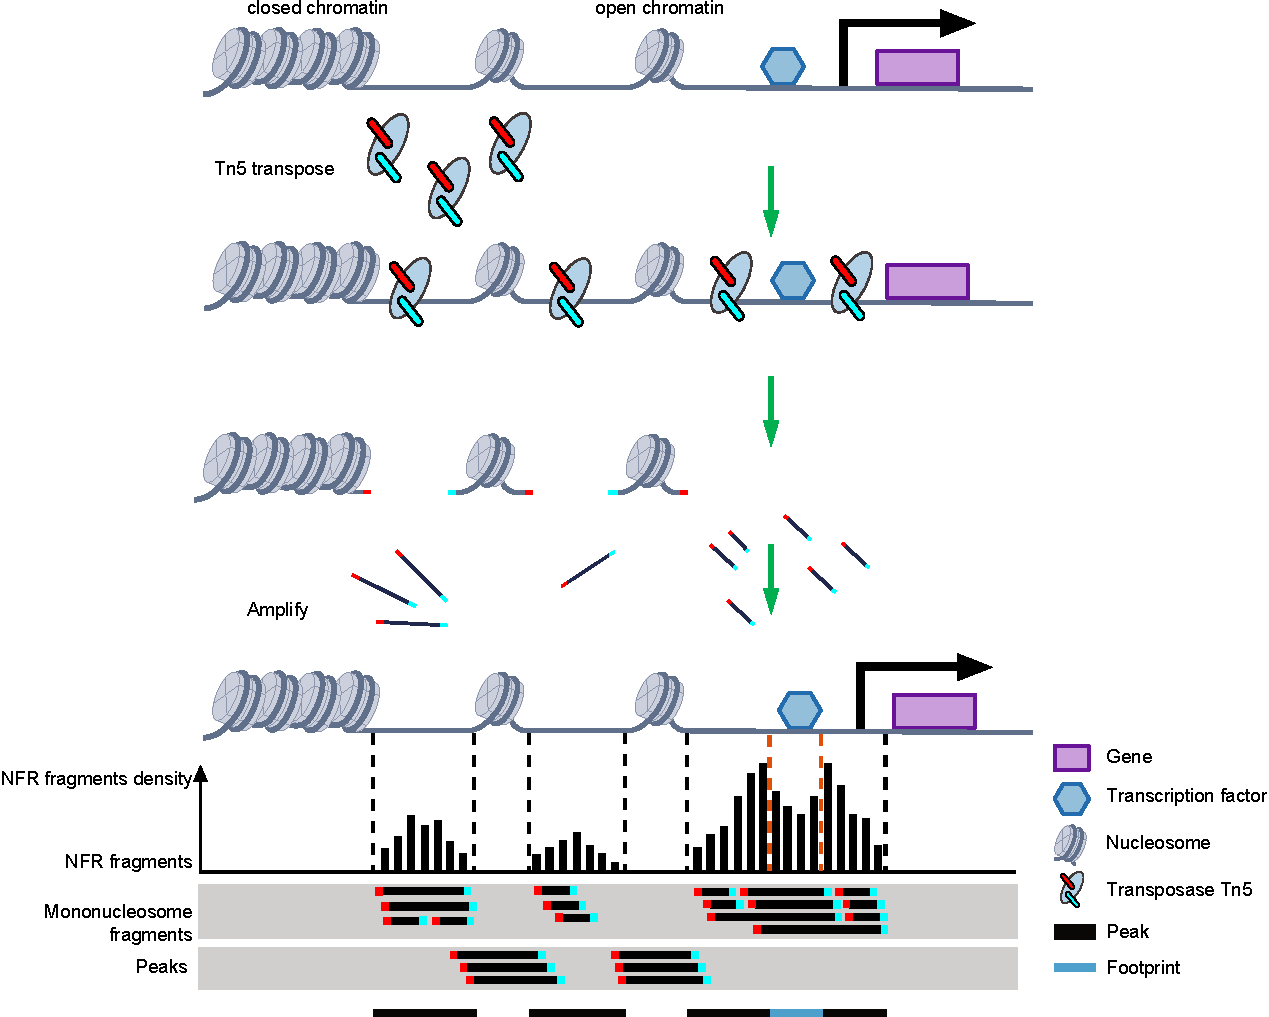
\includegraphics[width=0.85\textwidth]{scATAC-seq/fig}
	\vspace{0.1cm}
	\caption[ATAC sequenceing schematic flow.]{The ATAC-seq assay is employed for the identification of chromatin accessibility. Initially, the hyperactive Tn5 transposase selectively targets and modifies DNA regions characterized as "open" chromatin. Through a process known as tagmentation, the enzyme introduces sequencing adapters~(or priming sequences) into these open regions. Next, the resulting DNA fragments are amplified and input to high-throughput sequencing. \emph{Source:~\cite{yan2020reads}}~(modified to fit thesis format and/or clarify key points)}
	\label{fig:ATAC-seq}
\end{figure}

Protocols for single-cell ATAC-sequencing~(scATAC-seq) was introduced in 2015~\citep{Buenrostro2015,cusanovich2015multiplex}, enabling the unbiased identification of cell-type-specific regulatory elements within heterogeneous cell populations. Droplet-based scATAC-seq boasts a high throughput, capable of processing tens of thousands of cells per assay. Specifically, single nuclei are initially isolated from a single-cell suspension and subjected to bulk transposition with transposase Tn5. Following this, gel beads in emulsion~(GEM) are generated, with each gel bead being barcoded. Barcoded DNA fragments in droplets are finally used to create indexed libraries for high-throughput sequencing. Due to the advantages of high throughput and low costs for droplet-based single-cell ATAC-seq technology, the method is increasingly popular and has been commercialized by 10$\times$ Genomic(Chromium Next Gem Single Cell ATAC-seq Library Kit)~\citep{satpathy2019massively}.



%\subsection{Protein profiling in single cell}
%\label{background:sec1:protein}
%%Protein analysis at the single-cell level has relied on the use of antibodies that bind specifically to target proteins. Flow cytometry uses fluorescently labeled antibodies to convert protein signals into fluorescence signals~\citep{@article{kim2022single}
%Secreted proteins play crucial roles in facilitating diverse biological processes, including cell–cell communication, differentiation, migration, and maintaining homeostasis at the population or tissue level. Methods for directly measuring specific protein-secreting cells in clinical settings include enzyme-linked immunospot~(ELISPOT) and its variants, such as fluorescence-based immunospot~(FluoroSpot)~\citep{perfetto2004seventeen, karlsson2003comparison}. Indirect assessment of protein secretion function can be conducted through intracellular staining using fluorescence-activated cell sorting~(FACS)~\citep{bonner1972fluorescence}. The detection of multiple cytokines in single cells has become possible through intracellular cytokine staining using multicolor flow cytometry~\citep{irish2004single,hale2009stage}. Mass cytometry is a deviation from traditional flow cytometry utilizing mass spectrometry for detection via rare earth metal probes, has demonstrated highly multiplexed measurement of surface and intracellular proteins~\citep{spitzer2016mass}.
%
%To comprehensively assess the expression patterns of individual proteins, researchers typically opt for mass spectrometry or flow cytometry rather than sequencing~\citep{kim2022single}. The application of mass spectrometry to single-cell proteomics poses technical challenges related to factors like required sample amounts and detection coverage. Efforts are underway to develop methods that enable the measurement of more protein molecules with lower sample input. In recent single-cell studies, CyToF, a mass cytometry-based method, has been employed to analyze dozens of surface and intracellular proteins using metal-labeled antibodies. Particularly beneficial for immune cells, profiling cell surface proteins aids in cell type classification. CyToF has been extensively utilized in studies, including those in general and cancer immunology, often in conjunction with scRNA-seq analysis~\citep{kashima2020single}.





\begin{figure}[!ht]
	\centering
	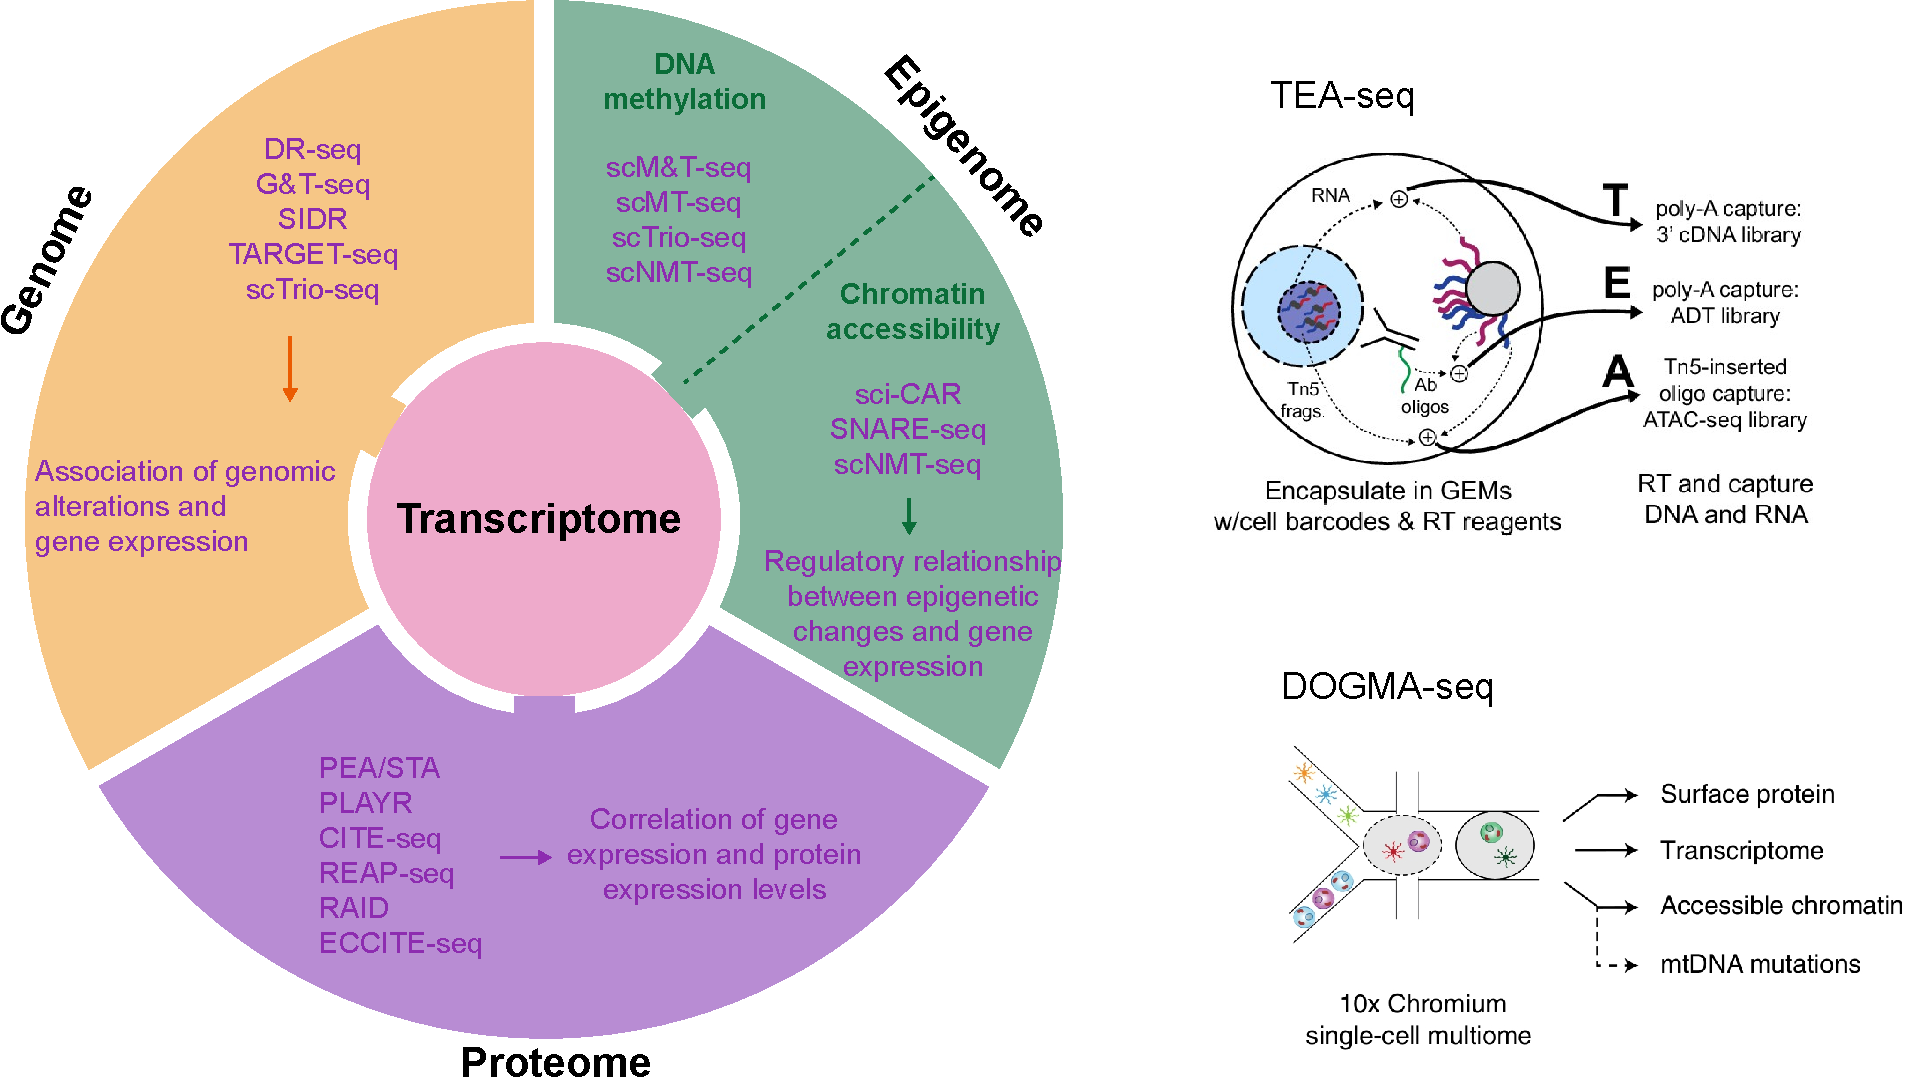
\includegraphics[width=0.50\textwidth]{multi-model-methods/fig}
	\vspace{0.1cm}
	\caption[multimodal methods protocols for Transcriptome, Genome, EpiGenome and Proteome]{multimodal methods protocols for Transcriptome, Genome, EpiGenome and Proteome. \emph{Source:~\cite{lee2020single}}~(modified to fit thesis format and/or clarify key points)}
	\label{fig:piechart-mulitmodal-methods}
\end{figure}



\subsection{Simultaneous multi-modal profiling of single cell}
\label{background:sec1:mulitmodal}
Single-cell multi-modal technologies typically analyze various types of molecules within a single cell, providing a more profound understanding of biology compared to studying individual molecular layers from separate cells. These advanced technologies unveil cellular heterogeneity across multiple molecular levels within a cell population, offering insights into the interconnectedness or independence of variation across different modalities. The datasets produced by these techniques hold the potential to facilitate a more comprehensive comprehension of the fundamental biological processes and mechanisms that contribute to cellular heterogeneity. Furthermore, they shed light on the associations between normal development, aging, disease etiology, and the intricate links between these phenomena. A variety of single cell multi-modal profiling methods have been proposed recently as shown in \tref{tab:multimodal-methods} and in \fref{fig:piechart-mulitmodal-methods}. We introduce these protocols by breaking down them into 3 groups:

\begin{itemize}
	\item \textbf{Transcriptome \& epigenome:}
	Several sequencing methods have been devised to simultaneously profile transcriptome and epigenome, E.g., single-cell combinatorial indexing chromatin accessibility and mRNA~(sci-CAR)~\citep{cao2018scicar}, single-nucleus chromatin accessibility and mRNA expression sequencing~(SNARE-seq)~\citep{chen2019SNARE}, and single-nucleus chromatin accessibility and RNA expression sequencing~(SHARE-seq)~\citep{ma2020shareseq}.


	\item \textbf{Transcriptome \& proteome:}
	Various methods have been developed, including proximity extension assay/specific RNA target amplification~(PEA/STA), proximity ligation assay for RNA~(PLAYR), cellular indexing of transcriptomes and epitopes by sequencing~(CITE-seq)~\citep{stoeckius2017citeseq}, and RNA expression and protein sequencing assay~(REAP-seq)~\citep{peterson2017reapseq}. Additionally, expanded CRISPR-compatible cellular indexing of transcriptomes and epitopes by sequencing~(ECCITE-seq)~\citep{mimitou2019ECCITE} is a modification and extension of CITE-seq, incorporating transcriptome, protein, clonotype, and CRISPR perturbation data at a single-cell resolution. To note, for the most common protocol CITE-seq, the sequencing data includes specific CITE-seq barcodes, also known as antibody-derived tags~(ADT), which identify the antibodies bound to the cells and provide information about the cell-surface proteins present~\citep{stoeckius2017citeseq}.

	\item \textbf{Transcriptome \& epigenome \& proteome:}
	Methods have been developed to profile more than two modalities, including TEA-seq~\citep{swanson2021simultaneous}, designed as a trimodal assay that simultaneously measures transcriptomics~(scRNA-seq), epitopes, and chromatin accessibility~(scATAC-seq) from thousands of single cells. Another method, DOGMA-seq~\citep{mimitou2021scalable}, can measure all features of TEA-seq and also detect mtDNA mutations simultaneously.

\end{itemize}

\begin{table}[!ht]
	\footnotesize
	\centering
	\begin{tabular}{lll}%{0.1\linewidth}}
		\toprule
		{\textbf{Modalities}} & {\textbf{Protocols}} & {\textbf{reference}} \\
		\midrule
		\multirow{5}{*}{\shortstack[l]{
\includegraphics[scale=1]{multi-model-methods/Protein_RNA.pdf}}}
		  & PLAYR & {~\cite{frei2016playr}} \\
		  & CITE-seq & {~\cite{stoeckius2017citeseq}} \\
      & REAP-seq & {~\cite{peterson2017reapseq}}\\
      & RAID & {~\cite{Gerlach2019RAID}} \\
		  & ECCITE-seq & {~\cite{mimitou2019ECCITE}}\\
		\midrule
		\multirow{5}{*}{\shortstack[l]{
\includegraphics[scale=1]{multi-model-methods/RNA_ATAC.pdf}}}
		  & sci-CAR & {~\cite{cao2018scicar}}\\
      & SNARE-seq & {~\cite{chen2019SNARE}} \\
      & scNMT-seq & {~\cite{clark2018scnmt}}\\
		  & scCAT-seq & {~\cite{liu2019scCAT}} \\
		  & SHARE-seq & {~\cite{ma2020shareseq}}\\
		\midrule
		\multirow{5}{*}{\shortstack[l]{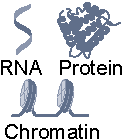
\includegraphics[scale=1]{multi-model-methods/3.pdf}}}
		& TEA-seq & {~\cite{swanson2021simultaneous}}\\
		& DOGMA-seq &~\cite{mimitou2021scalable} \\
		\\
		\\
		\\
		\bottomrule
	\end{tabular}
	\vspace{0.1cm}
	\caption[Major multimodal methods]{major multimodal methods.}
	\label{tab:multimodal-methods}
\end{table}


\section{Computational analysis of single cell}
\label{background:computational_singlecell}
After designing the experiment and conducting the sequencing, the subsequent crucial step involves performing computational analysis to extract valuable insights from the single cell data. For scRNA-seq and scATAC-seq data, the initial step involves aligning the reads to the reference genome to identify gene expression or the location of the reads, respectively. Generally, after obtaining the feature count matrix~(features by cells), the analysis includes three steps: pre-processing for quality checks and normalization, dimensional reduction and clustering to identify heterogeneous population groups, and downstream analysis based on different feature properties. In this section, we will introduce these analyses by first discussing the alignments of scRNA-seq and scATAC-seq. Next, we describe the computational analysis of scRNA-seq, followed by the analysis of scATAC-seq data and that of the surface protein data.

\subsection{Alignment}
\label{background:sec2:alignment}
The first step in the computational analysis of ATAC-seq/RNA-seq is the alignment, in which, raw sequencing reads~(DNA for scATAC-seq, RNA for scRNA-seq) are aligned to the reference genome to ensure these reads are located in the most probable position of the reference genome. This is typically accomplished by constructing a large index database from a reference genome and/or the set of reads, identifying potential regions for pairwise alignment~\citep{alser2021alignment}. The most widely used aligners are Bowtie2~\citep{langmead2012bowtie2}, BWA~\citep{li2009BWA} and STAR~\citep{dobin2013star}. These tools are utilized in the Cell Ranger ATAC/RNA/ARC pipeline developed by 10$\times$ Genomics.

\subsection{Computational Analysis of Single Cell RNA-seq}
\label{background:sec2:scRNA}
We will outline the computational workflow for scRNA-seq data analysis, covering preprocessing~(quality control, normalization, feature selection), core analysis~(dimensionality reduction, batch correction, and clustering), and downstream analysis~(differential expression, cell annotation, trajectory analysis, and gene set enrichment).

\begin{figure}[!ht]
	\centering
	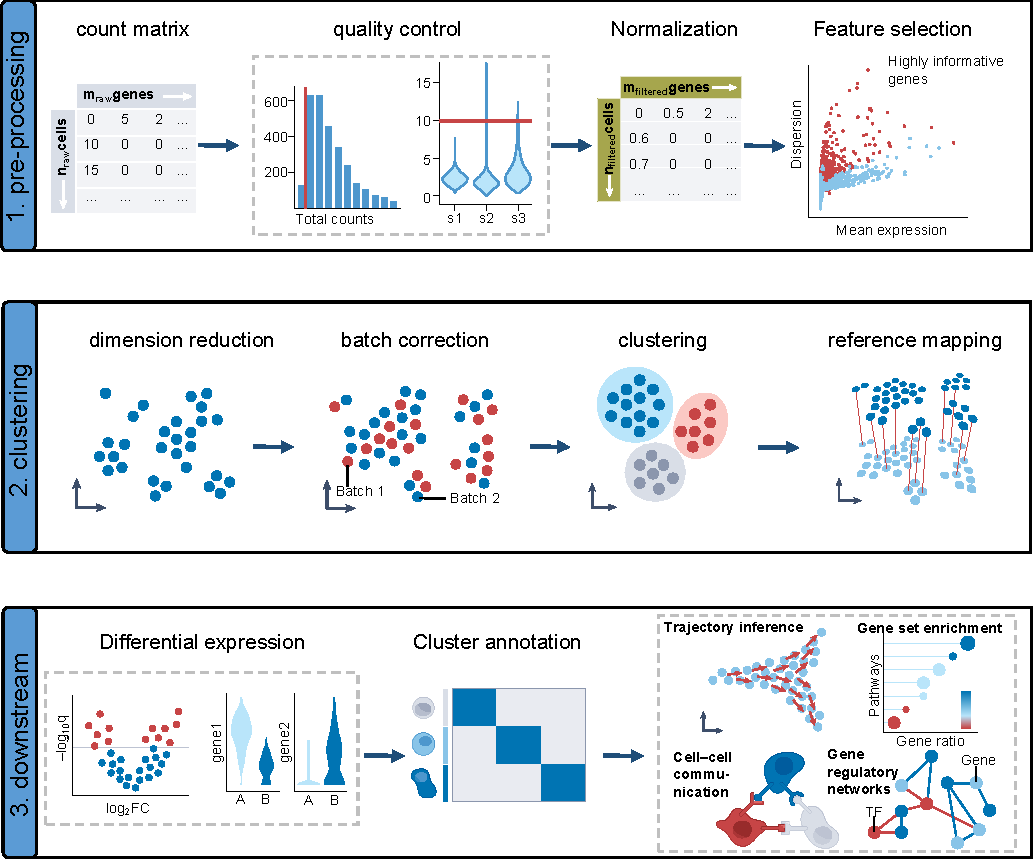
\includegraphics[width=0.85\textwidth]{workflow_scRNA/fig}
	\vspace{0.1cm}
	\caption[A common computational scRNA-seq analysis workflow]{
		\textbf{A common computational scRNA-seq analysis workflow}.
		\textbf{Step1:} Preprocessing starts with cell by gene count matrix, including quality control, normalization and feature selection.
		\textbf{Step2:} core analysis, including dimensionality reduction, batch correction and clustering and reference mapping.
		\textbf{Step3:} Downstream analysis, including differential expression, cell annotation, trajectory analysis and geneset enrichment.
	workflow scRNA. \emph{Source:~\cite{heumos2023best}}~(modified to fit thesis format and/or clarify key points)}
	\label{fig:workflow_scRNA}
\end{figure}

\subsubsection{Pre-processing}
We start from a count matrix where the mRNA sequence reads obtained are aligned to genes and cells of origin through an alignment pipeline e.g 10$\times$ cellranger pipeline~\citep{zheng2017massively}. The pipeline utilizes either cellular barcodes or unique molecular identifiers~(UMIs) in conjunction with a reference genome. We eventually obtain a count matrix representing cells by genes.
\begin{description}
	\item[Quality Control]
	We focus on droplet-based scRNA data quality control. \fref{fig:QCcells}A shows an intact droplet, where a droplet includes a cell and barcode bead to mark the cell ID. The objective of quality control is to filter low-quality cells~(\fref{fig:QCcells}B-E) and correct the noise. Cells characterized by a low number of detected genes, a shallow count depth, and a high proportion of mitochondrial counts are commonly referred to as low-quality cells. This designation is often indicative of cells in a state of decline, potentially exhibiting compromised membranes associated with cell damage or death. Low-quality cells are detected and filtered by manually setting thresholds, as suggested in a guide~\citep{luecken2019current}. Doublets or multiplets occur when more than one cell is present in a droplet~(\fref{fig:QCcells}D). The simplest method to address this issue is to filter out cells with an excessively high total count of gene molecules~(UMI). More sysmatic approach involves creating synthetic doublets by combining two cells and examining the neighborhoods of cells to detect potential doublets~\citep{mcginnis2019doubletfinder}. Ambient RNA removal typically involves using the expression profile of empty droplets to eliminate background noise from cells~\citep{janssen2023benchambient}.


	\item[Normalization]
	Cells may exhibit varying numbers of gene counts due to disparities in cell size or random variations during sequencing. Count normalization is employed to ensure comparability in cellular profiles. A common normalization method involves dividing the raw UMI count by the total detected RNAs in each cell, multiplying the result by a scaling factor~(typically set at 10,000), adding a pseudo-count~(usually 1), and subsequently applying a log transformation to the outcome. This size-factor normalization effectively mitigates technical variations arising from sequencing depth, while the log transformation serves to alleviate the impact of expression outliers. This approach is particularly valuable in preventing high-abundance genes from disproportionately influencing downstream analyses due to their elevated technical variability. Log-normalization is the default method in the most popular single cell analysis toolkit Seurat~\citep{stuart2019seurat3} written in R and Scanpy~\citep{wolf2018scanpy} implemented in python.

	\item[Feature Selection]
	Single-cell RNA-seq datasets typically contain more than 20,000 genes. Numerous genes lack informativeness and predominantly consist of zero counts. Thus, feature selection is necessary to select the most informative features(usually 3,000~5,000 genes) and reduce the computing resources and data dimensions, as well as alleviate issues such as model overfitting in downstream analysis~\citep{yang2021feature}. The objective is to exclude uninformative genes that may not reflect meaningful biological variation across samples. The commonly used method is implemented in Seurat, where genes are categorized based on their average expression. The gene with the highest ratio of variance to mean within each group is selected as the Highly Variable Gene~(HVG) for that specific bin~\citep{stuart2019seurat3}.
\end{description}

\begin{figure}[!ht]
	\centering
	\includegraphics[width=0.65\textwidth]{QC_cells/fig}
	\vspace{0.1cm}
	\caption[Droplets-based sequencing of cells in low quality.]{\textbf{Droplets-based sequencing of cells in low quality.} Droplet-based protocols for single-cell analysis require rigorous quality checks to ensure accurate downstream analysis. \textbf{A)} An intact droplet should ideally contain a single cell and a corresponding barcode for cell identification. \textbf{B)} Contamination may occur through the introduction of ambient RNA, leading to the inclusion of extraneous RNA reads not originating from the targeted cell. \textbf{C)} Droplets capturing dying cells typically exhibit lower levels of detected RNA reads, indicating compromised cell integrity. \textbf{D)} Occasionally, a droplet may capture more than one cell, posing challenges for subsequent analysis. \textbf{E)} Empty droplets, which capture no cells with extremely few gene expressions, are easily identified and can be excluded from analysis. These considerations emphasize the importance of thorough quality control measures in droplet-based single-cell protocols to ensure the reliability and accuracy of the generated data. \emph{Source:~\cite{heumos2023best}}~(modified to fit thesis format and/or clarify key points)}
	\label{fig:QCcells}
\end{figure}
\subsubsection{Dimensional reduction and clustering}
\label{background:sec2:dr_n_clustering}
\begin{description}
	\item[Dimensional Reduction]
	Dimensional reduction serves a dual purpose: preserving distances between cells with lower dimensions and facilitating data visualization. In the context of single-cell RNA sequencing~(scRNA-seq), Principal Component Analysis~(PCA)~\citep{hotelling1933pca} is often employed to reduce dimensionality, transforming high-dimensional data by maximizing the residual variance captured in each potential dimension. Subsequently, Uniform Manifold Approximation and Projection~(UMAP) or t-distributed Stochastic Neighbor Embedding~(t-SNE) are commonly utilized for data visualization with 2 dimensions preserved. However, both methods do not accurately represent the real distances between cells and should not be used for downstream analysis~\citep{mcinnes2018umap, van2008tsne}.

	\item[Batch Correction]
	Batch effects are a common confounding factor in single-cell RNA-seq experiments. Namely, they are systematic differences in measurements between batches~(e.g., technical replicates, different days of lab work, different individuals, etc.) that are not due to the biological signal of interest. Batch effects can be caused by a variety of factors, including differences in reagents, equipment, and personnel. Numerous methods have been proposed to address batch effects. Seurat employs canonical correlation analysis~(CCA) to identify anchors between batches, utilizing these anchors for subsequent correction~\citep{stuart2019seurat3}. Scanpy uses batch-balanced k-nearest neighbors~(BBKNN) to identify mutual nearest neighbors across batches, facilitating batch effect correction~\citep{polanski2020bbknn}. Harmony addresses batch effects by iteratively clustering similar cells from different batches at each iteration, maximizing batch diversity within clusters, and calculating correction factors for subsequent application~\citep{korsunsky2019harmony}. Comparative evaluations of batch correction methods indicate Harmony's superior performance~\citep{tran2020benchmark}.

	\item[Clustering]
	With the batch-corrected data, we can proceed to cluster cells into groups with similar expression profiles, elucidating the heterogeneity in the dataset. Various methods have been proposed for clustering, with graph-based clustering being particularly popular. For instance, Seurat utilizes the Louvain algorithm as its default clustering method~\citep{stuart2019seurat3}, while Scanpy defaults to the Leiden algorithm~\citep{traag2019louvain}. An independent benchmarking study of clustering methods revealed that SC3~\citep{kiselev2017sc3} and Seurat demonstrated the overall best performance and were the only ones to accurately recover cell types in droplet-based datasets~\citep{duo2018benchclustering}.

\end{description}

\subsubsection{Downstream analysis}
\begin{description}
	\item[Differential Gene Expression]
	Differential gene expression aims to identify genes that exhibit significant expression differences between clusters or conditions. These genes contribute valuable information for annotating cell types within clusters and interpreting biological distinctions influenced by specific conditions. The Wilcoxon rank-sum test stands out as the most widely used method for identifying differentially expressed genes, with the Student's t-test occasionally employed for this purpose. Other models, such as MAST, utilize the hurdle model to identify differentially expressed genes~\citep{finak2015mast}. Popular single-cell RNA analysis toolkits like Seurat and Scanpy have incorporated various statistical methods, including the Wilcoxon rank-sum test, t-test, and linear models like logistic regression, to identify genes exhibiting differential expression.

	\item[Cluster Annotation]
	With the clusters and significant gene markers of each cluster, identifying the cell types of each cluster is essential, requiring domain knowledge and an understanding of the biological context. The most prevalent approach to annotating cell types involves using marker genes—genes that exhibit high expression levels in specific cell types. Biologists can curate marker genes by identifying genes significantly highly expressed through differential gene expression analysis, aiding in the annotation of heterogeneous cell groups. Cluster annotation stands as a pivotal task in single-cell analysis, playing a crucial role in identifying cell types and interpreting the biological meaning of distinct cell groups.

	\item[Trajectory Inference]
	Trajectory inference, also known as pseudotemporal ordering, is a computational technique employed in single-cell transcriptomics to elucidate the pattern of a dynamic process undergone by cells. Trajectory inference arranges cells based on their progression through the identified process. Note that various subtasks of trajectory inference have been addressed by researchers, with dimension reduction being a critical aspect. Exclusive dimension reduction is essential due to the potential distortion of the global structure by nonlinear visualization methods like t-SNE and UMAP. Approaches such as multidimensional scaling~(MDS)~\citep{torgerson1952multidimensional} aim to reduce dimensions while preserving distance information in a 2 dimensional space, and diffusion maps~\citep{coifman2006diffusion} utilize Gaussian affinities to capture both local and global structural details. PHATE, developed by~\cite{moon2017phate}, leverages both local and global structure. Palantir employs a forced-directed layout to Gaussian affinities within a graph. Pseudotime simulation is another aspect focused on capturing the temporal order of differentiating cells. Diffusion pseudotime~(DPT), introduced by~\citep{haghverdi2016dpt}, measures transitions between cells using diffusion-like random walks and has been integrated into the popular Python single-cell toolkit Scanpy~\citep{wolf2018scanpy}. Additionally, methods like slingshot~\citep{street2018slingshot} and STREAM~\citep{chen2019stream} are explored in more detail in \sref{background:sec2:TI}.

	\item[Gene set Enrichment]
	Gene set enrichment analysis facilitates the summarization of numerous molecular insights into interpretable terms, such as pathways, which are defined as sets of genes known to be involved based on previous studies. Commonly used databases for this purpose include MSigDB~\citep{liberzon2011msigdb}, Gene Ontology~\citep{gene2004go}, KEGG~\citep{kanehisa2007kegg}, and Reactome~\citep{fabregat2018reactome}.
\end{description}

\subsection{Computational Analysis of Single Cell ATAC-seq}
\label{background:sec2:scATAC}
In many cases, single-cell ATAC-seq data analysis is similar to single-cell RNA-seq, with some distinctions due to feature differences present in scATAC. Firstly, the features, represented as a cell-by-peak matrix, are typically more sparse and have a larger feature space~(\fref{fig:modalities_differences}). This necessitates different strategies for feature normalization, feature selection, and dimensional reduction. Secondly, scATAC-seq features are not gene expressions, posing a challenge for cell annotation and data interpretation. Lastly, due to these feature differences, the biological insights obtained from scATAC-seq differ from those of scRNA-seq, giving rise to different downstream analyses like linkage analysis or motif discovery.

We will describe the computational workflow for scATAC-seq data analysis, including, feature matrix construction, preprocessing(feature definition, quality control, feature selection), core analysis~(dimensionality reduction, batch correction and clustering), and downstream analysis~(differential accessibility, trajectory inference etc. ).

\begin{figure}[!ht]
	\centering
	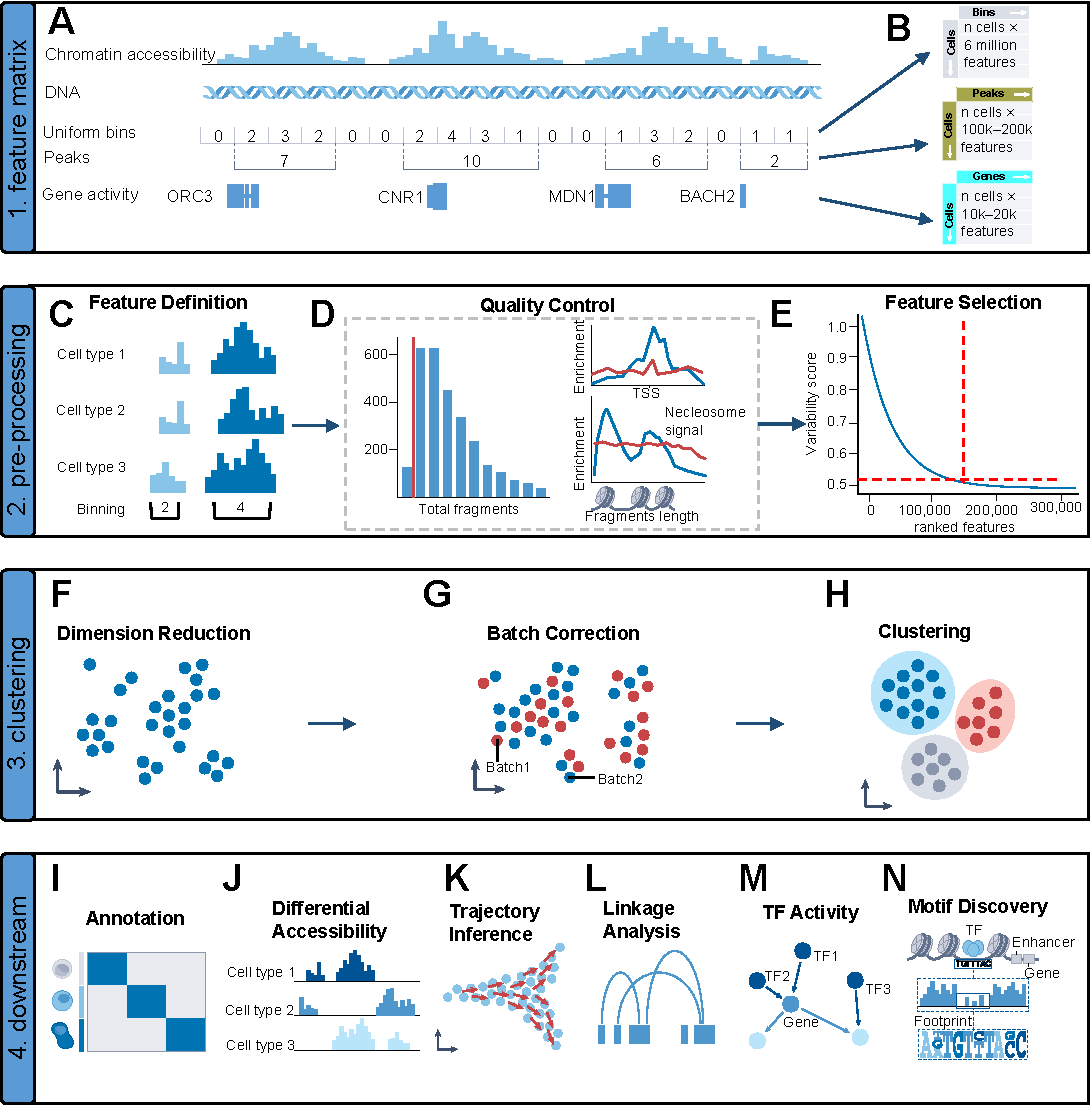
\includegraphics[width=0.85\textwidth]{workflow_scATAC/fig}
	\vspace{0.1cm}
	\caption[A common computational scATAC-seq analysis workflow]{
	\textbf{A common computational scATAC-seq analysis workflow:}
	\textbf{Step1:} Feature matrix construction using peaks, bins or gene accessibility.
	\textbf{Step2:} Preprocessing including feature selection, quality control, and feature selection.
	\textbf{Step3:} Core analysis including dimensional reduction, batch correction, clustering, label transferring, and cell type annotation.
	\textbf{Step4:} Downstream analysis including differential accessibility, trajectory inference, linkage analysis, TF activity and Motif discovery.

	\emph{Source:~\cite{heumos2023best}}~(modified to fit thesis format and/or clarify key points)}
	\label{fig:workflow_scATAC}
\end{figure}

\subsubsection{Feature matrix construction}
\label{background:sec2:scATAC:matrixconstruction}
In contrast to scRNA-seq data, which relies on clearly defined gene features, scATAC-seq data lacks a standardized feature set owing to the genome-wide nature of the data. Here we present three ways of feature matrix construction~(\fref{fig:workflow_scATAC}A). Most workflows typically utilize a cell-by-peak or cell-by-bin matrix as a foundation for analysis~\citep{heumos2023best}. However, it's important to note that the feature number in single-cell ATAC-seq is significantly larger compared to scRNA gene expression, usually reaching around 100,000 for this type of feature~(\fref{fig:modalities_differences}A). Another feature matrix gene activity score matrix can also be created to approximate gene expression, facilitating the interpretation of the data. We will outline how to construct these three feature matrices:
\begin{description}
	\item[Peak Matrix]
	Cell-by-peak is the most prevalent features for scATAC-seq data analysis. Peaks denote variable regions of open chromatin characterized by an enrichment of Tn5 transposition events compared to background noise. Note that the identification of peaks requires an adequate number of cells. Therefore, challenges may arise when dealing with rare cell types. To improve the sensitivity of peak detection, it is beneficial to call peaks within clusters. This approach mitigates the risk of overlooking peaks in rare cell types that might otherwise be obscured by the noise from more prevalent cell types. Currently, the most frequently employed peak caller for ATAC-seq is MACS2~\citep{zhang2008macs2} which was originally developed for ChIP-seq data, MACS2 utilizes a dynamic Poisson distribution to account for local background biases in the genome, enabling effective peak detection. Another peak caller HMMRATAC~\citep{tarbell2019hmmratac} which is a Hidden Markov Model-based method for ATAC-seq, employs a ``decomposition and integration'' approach to identify open chromatin regions by learning relationships between layers of coverage signals in a single ATAC-seq dataset. To note, 10$\times$ cellranger pipeline delivers a default cell-by-peak matrix output~\citep{satpathy2019massively}. R scATAC-seq analysis tool Signac~\citep{signac} and Python tool Episcanpy~\citep{Danese2021episcanpy} use cell-by-peaks features to do the analysis.

	\item[Bin Matrix]
	To generate a cell-by-bin count matrix, the genome is segmented into uniform-sized bins(typically 500 bps). Single-cell ATAC-seq profiles are then represented as a cell-by-bin matrix, where each element indicates the number of sequencing fragments overlapping with a specific bin in a particular cell. This bin matrix is employed in scATAC-seq toolkits such as snapATAC~(~\citep{fang2021snapatac}) and ArchR~(~\citep{Granja2021}).

	\item[Gene Score Matrix]
	Gene activity score is a prediction of how highly expressed a gene will be based on the accessibility of regulatory elements in the vicinity of the gene. Signac~\citep{signac} extracts gene coordinates and extends them to include the 2 kb upstream region~(as promoter accessibility is often correlated with gene expression) and then counts the number of fragments for each cell that map to each of these regions. Whereas ArchR~\citep{granja2019single} creates a tile matrix using a user-defined tile size~(default is 500 bp), overlaps these tiles with the user-defined gene window~(default is 100 kb on either side of the gene), and then calculates the distance from each tile~(start or end) to the gene body, with optional extensions upstream or downstream, or to the gene start.
\end{description}

\subsubsection{Pre-processing}
\begin{description}
	\item[Quality control]
	Similar to single-cell RNA sequencing, the number of fragments per cell serves as a crucial metric for filtering low-quality cells in single-cell ATAC-seq. A low number of fragment reads suggests low-quality cells, while an excessively high number might indicate potential doublets. Additionally, the enrichment of transcription start sites~(TSS)~\citep{Granja2021} is commonly employed as a filtering criterion. Other metrics, such as the fraction of reads in peaks~(FRiP), the ratio of reads in promoter regions and the ratio of reads in blacklist sites, are also utilized for quality checks in scATAC-seq data. Empirically, for human and mouse data, common quality thresholds include requiring the number of unique nuclear fragments to be greater than 1000, ensuring the FRiP is greater than 0.3, and targeting TSS enrichment scores greater than 5 or 6. The threshold should be determined based on the characteristics of samples in practice. Doublets detection is also necessary for scATAC-seq data. ArchR~\citep{Granja2021} also implemented a doublets detection function. It generates synthetic doublets in silico by blending the reads from thousands of combinations of individual cells and finding their nearest neighbors to identify doublets whose signals closely resemble those of the synthetic doublets.

	\item[Normalization]
	For scATAC data, we typically employ the term-frequency inverse-document-frequency~(TF-IDF) method for normalization. This method transforms a cell-to-feature
	matrix by assigning greater weight to rarer peaks within the cell population. The resulting transformed data matrix tends to emphasize peaks that demonstrate higher variability, enhancing their informativeness for distinguishing between different cell types. Widely-used scATAC-seq toolkits such as Signac~\citep{signac} and ArchR~\citep{granja2019single} both utilize TF-IDF for normalizing the count matrix.


	\item[Feature Selection]
	Given the typically larger number of peaks compared to genes in scATAC-seq data, effective feature selection is crucial. A common approach involves selecting peaks with high variance across cells, with methods like Signac~\citep{signac} utilizing the variance of the TF-IDF transformed matrix for peak selection.
\end{description}
\subsubsection{Dimensional reduction and Clustering}
\begin{description}
	\item[Dimensional Reduction]
	Unlike the scRNA data, scATAC usually uses different strategies to reduce the dimensions. The most commonly used Latent semantic indexing~(LSI) was first introduced for the analysis of scATAC-seq data by~\citep{cusanovich2015multiplex}. It combines the steps of TF-IDF followed by Singular value decomposition~(SVD). Signac~\citep{signac} use LSI as the default dimension reduction method, whereas ArchR implemented Iterative Latent Semantic Indexing(iterativeLSI)~\citep{satpathy2019massively, granja2019single} which initiates by performing an initial Latent Semantic Indexing~(LSI) transformation on the most accessible bins and identified lower-resolution clusters that remain unaffected by batch confounding. To note, the first component of Latent Semantic Indexing~(LSI) in scATAC-seq data often captures sequencing depth. It is recommended to assess the correlation between each component and sequencing depth to exclude noise introduced for downstream analysis, as suggested by Signac~\citep{signac}. For visualization purposes, UMAP and t-SNE are considered optimal choices, similar to single-cell transcriptomics.

	\item[Batch Correction \& Clustering]
	Similar to scRNA, see \sref{background:sec2:dr_n_clustering}.


\end{description}
\subsubsection{Downstream analysis}
\label{background:sec2:atac_downstream}
\begin{description}

	\item[Annotation]
	Without gene expression features, it's a challenge to annotate the cell types of each cluster. One way is to transfer labels from previous studies to scATAC data. Typically, this is achieved by integrating scATAC with existing scRNA data. For instance, methods provided by Seurat~\citep{stuart2019seurat3} find shared nearest neighbors from different studies to transfer labels~\citep{stuart2019seurat3}. Another approach involves using multimodal data as a molecular bridge, facilitating the mapping of scATAC onto scRNA-seq references~\citep{hao2023dictionary}. Apart from label transferring, we can also use gene activity score~(\sref{background:sec2:scATAC:matrixconstruction}) differentiation to identify cell types for each cluster. The Transcription Factor(TF) motif enrichment score can be also used to assit the identification of the cell types.

	\item[Differential Accessibility]
	To gain insights into cluster/cell type-specific biology, one can perform differential accessibility analysis, akin to scRNA differential gene expression. Various statistical methods have been employed for this task, including the aforementioned Wilcoxon test from scRNA, which is also applicable here. Additionally, binomial tests~\citep{cusanovich2018single}, and logistic regression models~\citep{hao2021seurat4} are commonly used in scATAC-seq tools. Typically, methods for differential accessibility take into account the removal of technical biases, such as unique nuclear fragments and TSS enrichment. ArchR~\citep{Granja2021} selects a set of background cells that match the known biases for each cell group and performs comparisons between each cell group and its background cells. Signac~\citep{hao2021seurat4} employs logistic regression for differential accessibility analysis and treats the total number of fragments as a latent variable to mitigate the effects of technical biases.

	\item[Trajectory Inference]
	Trajectory analysis has been discussed in \sref{background:sec2:scRNA}.


	\item[Linkage Analysis]
	Accessibility profiles along the linear genome in individual cells have been shown to correlate with higher-order chromosome folding~\citep{Buenrostro2015}. Consequently, scATAC-seq data enables the extraction of promoter–enhancer interactions and gene regulatory networks through linkage analysis. Two main types of linkage analysis are peak-to-peak co-accessible analysis and peak-to-gene linkage analysis. Cicero~\citep{pliner2018cicero} is an algorithm designed for establishing genome-wide connections between distal enhancers and promoters based on co-accessibility patterns in scATAC-seq data. Peak-to-peak co-accessibility analysis seeks correlations of accessibility between two peaks across cells, but it doesn't necessarily indicate a direct regulatory relationship due to frequent co-accessibility of cell type-specific peaks. To overcome this, peak-to-gene linkage analysis integrates scRNA-seq data, calculating correlations between peak accessibility and gene expression~\citep{Granja2021}. This method, compared to peak-to-peak co-accessibility analysis, more accurately reflects gene regulatory interactions~\citep{shi2022scatacoverview}.

	\item[Motif Discovery]
	The binding of transcription factors to cis-regulatory DNA sequences controls gene expression programs and the dynamics during development or in disease. To compute transcription factor~(TF) binding site enrichment scores at the single-cell level, chromVAR~\citep{schep2017chromvar} assesses the accessibility deviation across all motif-containing peaks per cell while correcting for the Tn5 transposase's insertion bias. This bias arises from the sequence binding preferences of the transposase.

\end{description}

%%might ignore the surface protein part
\subsection{Computational Analysis of Single Cell Surface Protein}
\label{background:sec2:protein}
The feature size of surface protein is much smaller~(around 100) compared to other modality types~(\fref{fig:modalities_differences}A). It is often profiled together with scRNA-seq e.g., CITE-seq~\citep{citeseq2017} simulatenously profiles scRNA and suface protein.

Surface protein profilling outputs antibody-derived tags~(ADT) count matrix, which exhibits higher density compared to scRNA-seq and scATAC-seq data. For quality check, it is advisable to remove libraries with zero counts for the entire or a majority of the antibody panel~\citep{amezquita2020adtqc}. For protocols that simultaneously measure RNA and ADTs, such as CITE-seq~\citep{citeseq2017}, quality control for RNA and ADTs should be conducted separately. Since antibody efficacy can vary, batch correction of ADT data across multiple studies should also be performed~\citep{zheng2022adtqc}. To address biases in cell composition, normalization techniques such as centered log-ratio~(CLR) transformation is recommended~\citep{stoeckius2017citeseq}. The downstream analysis of ADT data follows a similar pipeline to unimodal RNA analysis, wherein annotated clusters can be tested for differential abundance.


%\section{Related works}
%\label{background:related_works}
\section{Computational Analysis of Single Cell Multimodal Omics}
\label{background:multimodal}
Computationally, multimodal single-cell omics profiling has paved the way for developing models that can capture interactions and associations among multiple modalities at single-cell resolution. In this section, We begin by presenting the common workflow of single-cell multimodal analysis. Following that, we delve into two crucial computational tasks: integration and trajectory inference for single-cell multimodal data. We will outline the challenges, current approaches, and our objectives to address these issues.

\subsection{Common Workflow of Single Cell Multimodal Omics}
\label{background:multimodal}
We will outline the computational workflow for the analysis of single-cell multimodal data. As depicted in \fref{fig:workflow_multimodal}, two crucial challenges, namely data integration and trajectory inference, need to be addressed during single-cell multimodal analysis.

\begin{figure}[!ht]
	\centering
	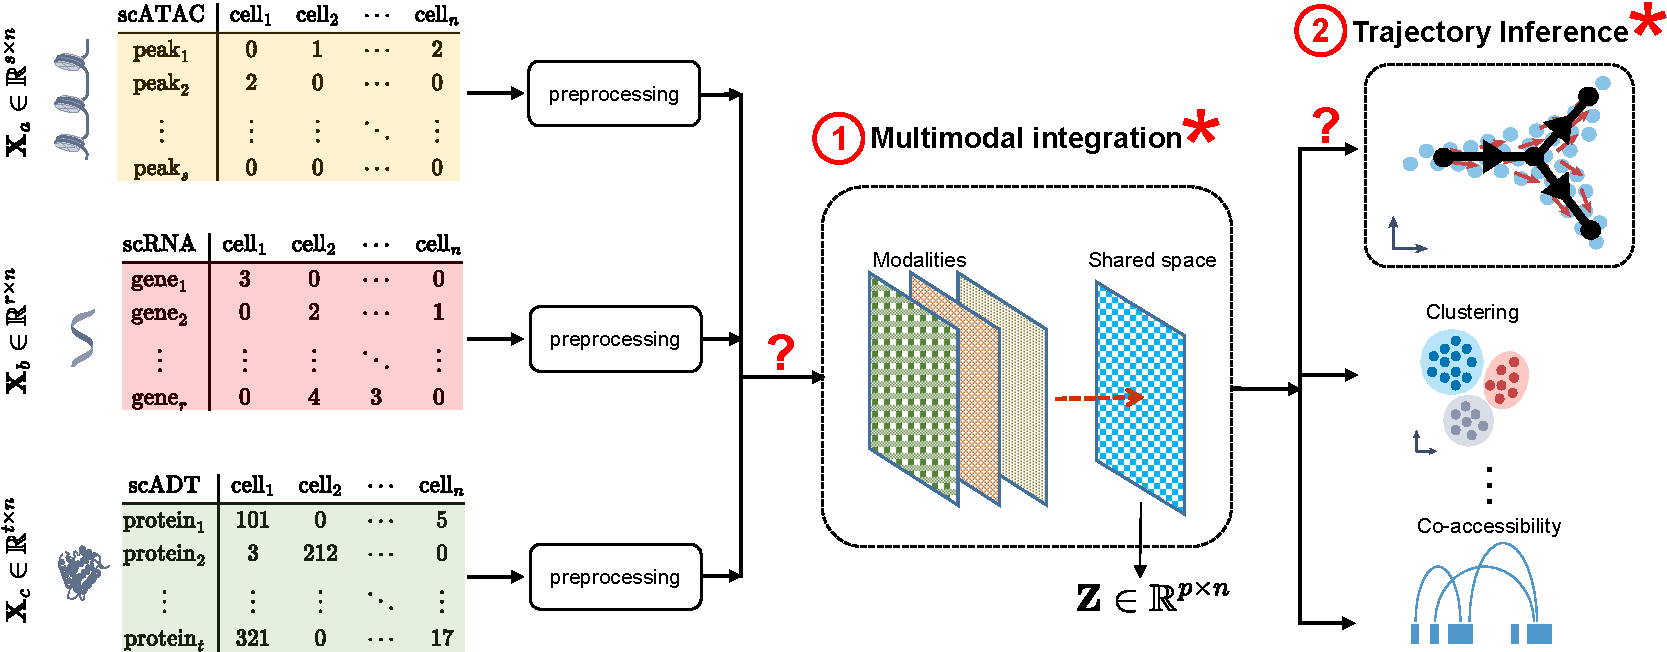
\includegraphics[width=0.95\textwidth]{workflow_multimodal/fig}
	\vspace{0.1cm}
	\caption[A common computational multimodal analysis workflow.]{A common computational workflow for single-cell multimodal dataset analysis involves several steps. Each count matrix from different modalities undergoes preprocessing, including quality checks and normalization. Subsequently, single-cell multimodal integration is performed to obtain a uniform latent space. Based on the latent space, downstream analyses can be conducted, such as clustering, trajectory inference, and visualization. Two key problems need to be addressed: \textcircled{\raisebox{-0.9pt}{1}} How to obtain a unified latent space for downstream analysis, and \textcircled{\raisebox{-0.9pt}{2}} Are there trajectory inference methods that can cooperate with multiple modalities?}
	\label{fig:workflow_multimodal}
\end{figure}

	%While many analyses developed for unimodal datasets can be adapted for multimodal data, establishing a consistent dimension reduction approach(data integration) is advantageous for subsequent analyses.

	As illustrated in \fref{fig:workflow_multimodal}, following the preprocessing steps for each modality, the subsequent objective is to integrate these modalities to derive a consistent latent space. This unified latent space facilitates downstream analyses, including trajectory analysis, clustering, and visualization. It is crucial to emphasize the importance of batch correction, particularly when working with multiple batches of data, prior to integration.

	In addition to the downstream analysis for unimodal data, the incorpoartion of multiple modalities can enhance specific tasks performed in unimodal analysis, leading to more profound insights, such as achieving more accurate Gene Regulatory Networks~(GRN). For instance, scMega~\citep{li2023scmega} utilizes scRNA-seq and scATAC-seq data to infer GRN. And the integration of scRNA-seq and proteomic data proves valuable for a detailed examination of signaling networks~\citep{heumos2023best}.


%\subsection{Challenge of single cell multi-modal integration and trajectory inference}
%\label{background:sec2:challenge}

\subsection{Single Cell Multimodal Integration}
We will discuss the computational challenge of integrating single-cell multimodal data, provide an overview of current methods for the task, and outline our objectives for addressing the limitations present in existing computational approaches to single-cell multimodal integration.
\subsubsection{Challenge of Single Cell Multimodal Integration}
\label{background:sec2:challenge_integration}
Single-cell multimodal profiling represents a nascent field, and the integration of single-cell multimodal data, while several tools have been developed for this purpose, still poses challenges:

\begin{itemize}
	\item \textbf{Heterogeneous statistical properties:}
	Different modalities exhibit distinct statistical properties, presenting a challenge for the integration of single-cell multimodal data. For instance, the feature size of single-cell surface proteins is typically around 100, while single-cell RNA-seq and single-cell ATAC-seq have feature sizes of 20,000+ and 100,000+~(\fref{fig:modalities_differences}A). The sparsity levels of the feature matrices for different modalities also vary significantly. For example, there are more than 10\% non-zero entries for scRNA-seq data, whereas scATAC-seq data has less than 3\% non-zero entries~\citep{li2021chromatin}, and surface protein data has more than 70\% non-zero entries~(\fref{fig:modalities_differences}B). Moreover, the feature distributions significantly differ among distinct modalities~(\fref{fig:modalities_differences}C). The substantial differences between modalities present a significant challenge in deriving a unified latent space that effectively incorporates all features without losing valuable information.


	\item \textbf{Modality Compatibility:}
	Increasingly, new protocols are being developed to simultaneously measure features in the same single cell, such as open chromatin, gene expression, protein, and DNA methylation. The combinations of different modality types present a challenge for integration; Certain methods, such as scAI~\citep{jin2020scai}, are designed to handle only two modalities, while others, like Liger~\citep{kriebel2022uinmf}, are restricted to specific feature matrices.

	\item \textbf{Scalability:}
	As sequencing costs decrease and technologies improve, we anticipate that multimodal datasets will follow a similar trend as single-cell RNA sequencing~(scRNA-seq), where in less than ten years, the size of experiments increased from the order of tens to millions of cells~\citep{svensson2018exponential}. More efficient methods are needed, ones that require less memory and reduced running time.

	\item \textbf{Interpretability:}
	Interpretation of each component of the latent space is essential to understand the information it captured in the latent space, some methods like Seurat WNN~\citep{hao2021seurat4} only delivered a network for the integration. When associating molecular features with the latent space, it's better if the method is capable of interpreting each component using features from specific modalities, and most methods lack this ability.

	\item \textbf{Removal of batch effects}:
	In single-cell multimodal integration, addressing heterogeneous features across different modalities is crucial, and the challenge extends to mitigating batch effects arising from both biological and technical sources. Certain methods, such as scAI~\citep{jin2020scai}, might be limited in their ability to incorporate external batch correction techniques, potentially leading to confounding results from combined batches and biological variations.

	\item \textbf{Validation}
	Evaluating the outcomes of data integration presents a significant challenge. In practice, there is no definitive ground truth, necessitating an evaluation based on downstream analysis tasks, such as assessing clustering agreement with true labels. However, these true labels, often annotations from a study, may introduce noise or inaccuracies in cell type identification. Therefore, a thorough validation should be applied to comprehensively assess the effectiveness of a method.

  \item \textbf{Execessive Presumption}
  Most methods either assume a specific data distribution or involve fitting the model with several parameters, requiring prior knowledge that may not be universally applicable. For example, Seurat WNN requires inputting the number of neighbors and scaling factor for the neighborhood, and MOFA involves several hyperparameters for model regularization. Moreover, MOFA requires manual selection of informative components for downstream analysis after obtaining the latent components. A method is needed to automatically identify the most important shared information across different modalities.

\end{itemize}

\begin{figure}[!ht]
	\centering
	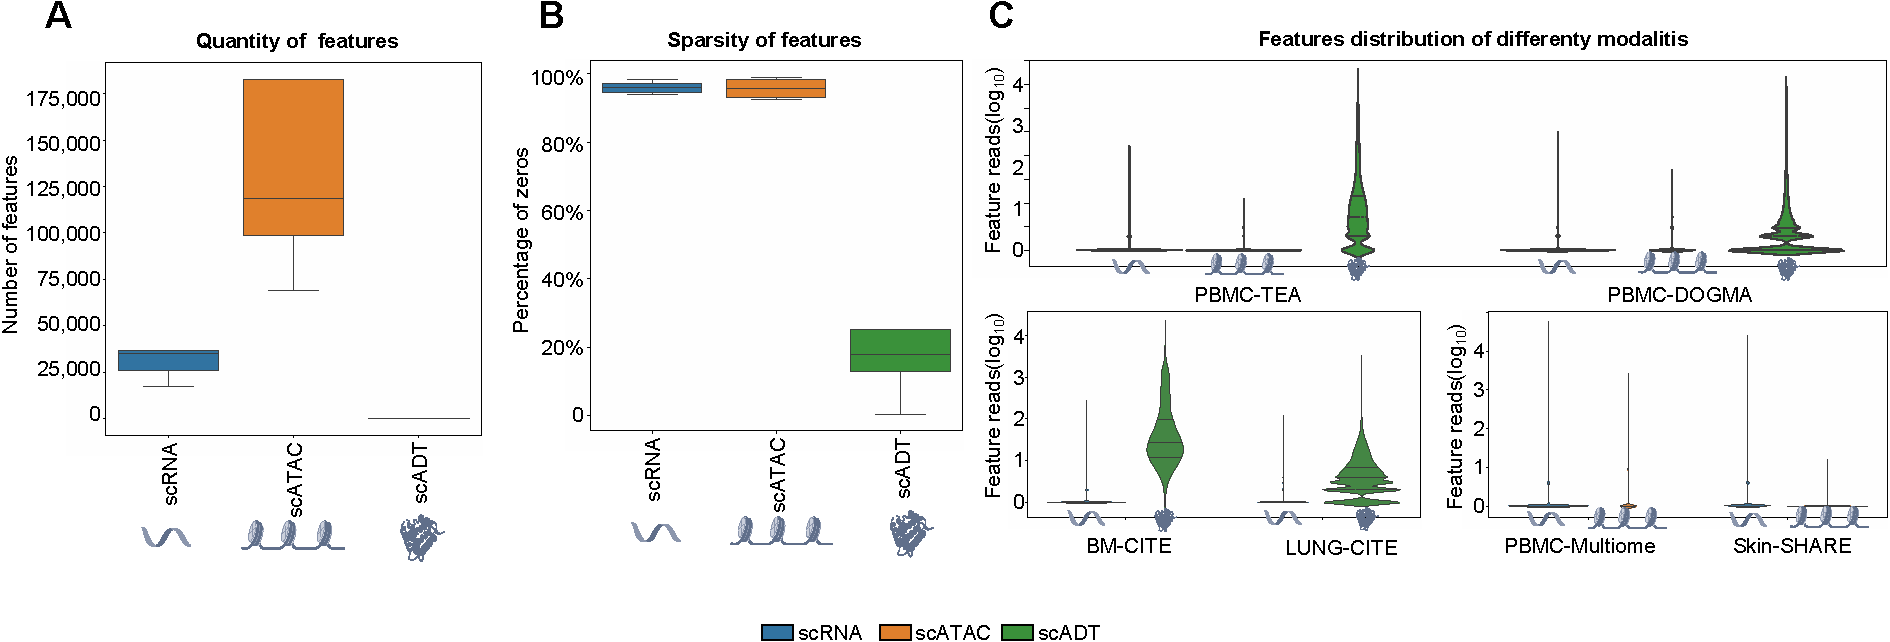
\includegraphics[width=0.95\textwidth]{feature_statistic/fig}
	\vspace{0.1cm}
	\caption[features characteristics comparison showing the challenge of multimodal integration.]{Illustration of six single-cell multimodal data. A) Number of features in scRNA, scATAC and scADT modalities. B) Percentage of zero entries in the three modalities, C) Element counts percentages in different modalities for the six single cell multimodal data.}
	\label{fig:modalities_differences}
\end{figure}

\subsubsection{Computational Methods for Single Cell Multimodal Integration}
\label{background:sec2:integration}
The challenges discussed in \sref{background:sec2:challenge_integration} regarding the integration of single-cell multimodal data pose difficulties in developing an efficient and effective integration method.

\begin{table}[!ht]
	\small
	\centering
	\begin{tabular}{llllll}
		\toprule
		Name & algorithm & modality types & \#modalities & Reference \\
		\midrule
    DIABLO & PLS-DA & universal & any & \cite{singh2019diablo}\\
    Liger & NMF & shared-features& 2 & \cite{kriebel2021nonnegative} \\
		MOFA   &  Matrix Factorization & universal & any &  \cite{argelaguet2020mofa+} \\
		Schema & Metrics learning  & universal & any & \cite{singh2021schema} \\
    scAI & Matrix Factorization & scRNA,scATAC & 2 & \cite{jin2020scai}\\
		Seurat WNN	 & WNN & universal & any & \cite{hao2021seurat4} \\
		\bottomrule
	\end{tabular}
	\vspace{0.1cm}
	\caption[Overview of computational integration methods]{Overview of computational integration methods.}
	\label{tab:methods_integration_overview}
\end{table}

Several methods have been developed to address this task, and we will now review the computational single-cell multimodal integration methods available in the literature. These methods can be classified into four groups based on the techniques they employ. The first group encompasses matrix factorization, which breaks down the multimodal count matrix into the product of two matrices. One matrix contains the latent factors representing the features, while the other incorporates the cells embedded in the latent factor space~(e.g., MOFA, scAI, Liger). The second group endeavors to construct a weighted nearest network that captures common information across all modalities~(e.g., Seurat WNN). The third group seeks to maximize the covariance or correlation between two modalities~(e.g., DIABLO, Symphony). The fourth group employs metric learning to reweigh modality features by maximizing their agreement with other modalities(Schema). \tref{tab:methods_integration_overview} summarizes the characteristics of each method.

\begin{description}
  \item[DIABLO]
  Data Integration Analysis for Biomarker discovery using Latent cOmponents~(DIABLO) is a generalization of sGCCA~\citep{tenenhaus2014variable}, which is a multivariate extension of canonical correlation analysis~(CCA). For $Q$ normalized and centered data matrices $X^1, \cdots, X^Q$ of dimensions $N\times D_q$, where $N$ denotes the number of cells and $D_q$ denotes the number of features. DIABLO aims to find a set of $H$ linear combinations of the $Q$ data matrices that are maximally correlated. The linear combinations are defined as:
  \begin{equation}
  \begin{aligned}
  	\underset{a_h^{(1)},\cdots,a_h^{(Q)}}{\max} \sum_{i,j=1, i\neq j}^Q c_{i,j} \text{cov}(X_h^{(i)} a_h^{(i)}, X_h^{(j)} a_h^{(j)}),\\
  	s.t. \|a_h^{(q)}\|_2 = 1, \text{ and } \|a_h^{(q)}\|_1 \leq \lambda^{(q)}, \text{for all} 1\leq q \leq Q.
  \end{aligned}
  \end{equation}
  Where $a_h^{(q)}$ is the variable coefficient vector for the $h$-th linear combination of the $q$-th data matrix, and $c_{i,j}$ is the weight of the correlation between the $i$-th and $j$-th data matrices. The first constraint is to normalize the linear combination, and the second constraint is to sparsify the linear combination. DIABLO solves the optimization problem by iteratively updating the $a_h^{(q)}$ and $c_{i,j}$ until convergence.


 \begin{figure}[!h]
  	\centering
  	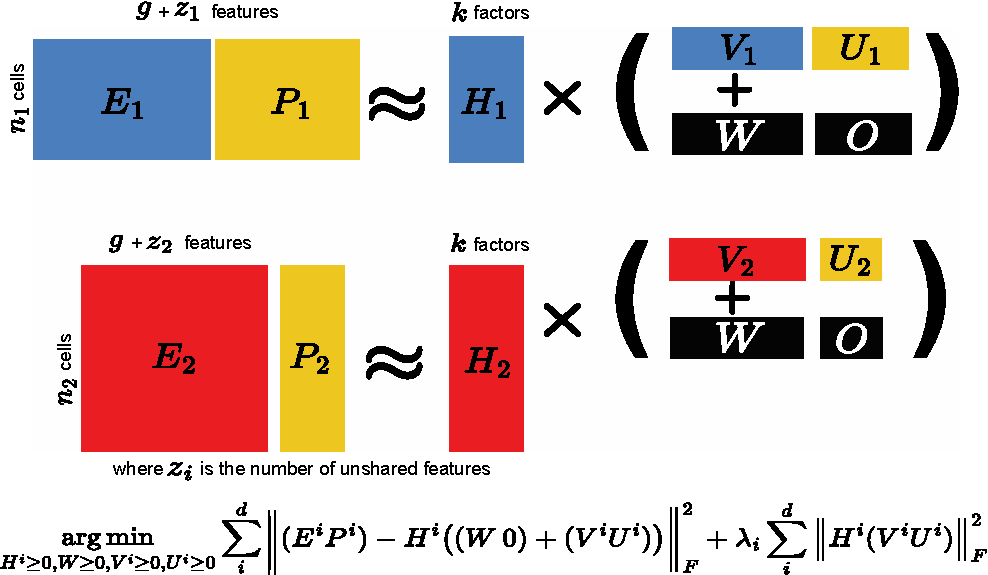
\includegraphics[width=0.6\textwidth]{Alg_Liger/fig}
  	\vspace{0.1cm}
  	\caption[Illustration of Liger integration competing method.]{\textbf{Illustration of Liger integration competing method.} Liger Schematic representation of the matrix factorization strategy~(top) and the formulation of the optimization problem~(bottom). The introduction of a factor matrix $U_i$ enables the utilization of unshared features in joint matrix factorization. Each dataset~($E_i$) undergoes decomposition into shared metagenes~($W$), dataset-specific metagenes constructed from shared features~($V_i$), unshared metagenes~($U_i$), and cell factor loadings~($H_i$). The inclusion of the U matrix enables unshared features occurring in only one dataset to contribute to the resulting integration. \emph{Source~\cite{kriebel2022uinmf}}~(modified to fit thesis format and/or clarify key points)
  }
  	\label{fig:Alg_Liger}
 \end{figure}

  \item[Liger]
  Linked Inference of Genomic Experimental Relationships(Liger)~\citep{kriebel2022uinmf} implemented UINMF algorithm, which uses iterative Non-negative Matrix Factorization~(iNMF) to learn a common latent space across multiple modalities. It allows the inclusion of both shared and unshared features across modalities to learn a common latent space. They incorporate intergenic peaks from snATAC-seq data and additional genes not measured in all datasets. For each data set $E^1, E^2, \cdots, E^n$, Liger first normalizes the data, and selects $m$ variable genes~(shared across all datasets), and $z_i$ variable features, such that after scaling $E^i \in R_{+}^{(m+z_i)\times n_i}\ (i=1,\cdots,N)$. Given $K$ and $\lambda_i$, the objective function is:
  \begin{equation}
	  \underset{H^i\geq 0,W\geq 0, V^i\geq 0, U^i \geq 0}{\arg\min} \sum_i^{d}\Big\| (E^i P^i) - H^i \big((W 0) + (V^i U^i)\big)\Big\|_{F}^2 + \lambda_i\sum_i^d\Big\|H^i(V^i U^i)\Big\|_{F}^2
  \end{equation}
  Liger uses coordinate block descent~(BCD) to solve the optimization problem, which derives the parameters into blocks and finds the optimal solution for each block iteratively~(\fref{fig:Alg_Liger}).


\begin{figure}[!h]
  	\centering
  	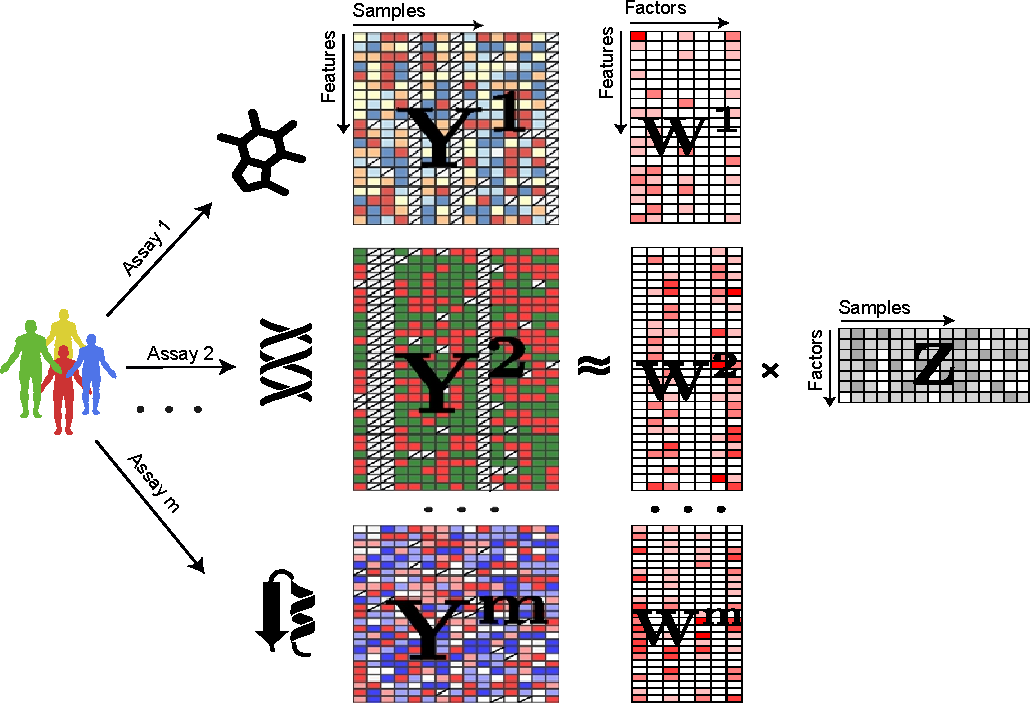
\includegraphics[width=0.65\textwidth]{Alg_MOFA/fig}
  	\vspace{0.1cm}
  	\caption[Illustration of MOFA integration competing method.]{\textbf{Illustration of MOFA integration competing method.} MOFA takes $m$ data matrices as input $Y_1, \cdots Y_m$, one or more from each data modality, with co-occurrent samples but features that are not necessarily related and that can differ in numbers. MOFA decomposes these matrices into a matrix of factors~($Z$) for each sample and $m$ weight matrices, one for each data modality~($W_1,\cdots, W_m$) where white cells in the weight matrices correspond to zeros~(i.e., inactive features). The cross symbol in the data matrices represents missing values. \emph{Source~\cite{tewari2017mofa}}~(modified to fit thesis format and/or clarify key points)
  }
  	\label{fig:Alg_MOFA}
\end{figure}
 
  \item[MOFA]
  Multi-Omics Factor Analysis+~(MOFA+)~\citep{argelaguet2020mofa+} uses Bayesian group factor analysis and variational inference to decompose individual modalities simultaneously by estimating a common latent factor matrix $Z$, as well as the weights for the transformation of the modalities to the latent space. MOFA+ includes a procedure to determine the optimal number of factors~(dimension of the latent space) and has several hyper parameters for model regularization, detection of number of factors and learning rates. Specifically, it decomposes simultaneous multimodal of $M$ data matrics $Y^1, \cdots, Y^M$ of dimensions $N\times D_m$, where $N$ denotes the number of cells and $D_m$ denotes the number of features, $G$ is the number of sample groups, and $N_g$ is the number of samples in the $g$th group and $K$ is the number of factors. The matrix decomposition is:
  \begin{equation}
  Y_{gm} = ZgW_m^{T} + \varepsilon_{gm},
  \end{equation}
  Where $Y_{gm}$ is the the matrix of observations for the $m$th data modality and the $g$th group, $Z_g$ is the matrix of latent factors for the $g$th group, $W_m$ is the matrix of weights for the $m$th data modality, and $\varepsilon_{gm}$ is the matrix of residuals. The latent factors $Z_g$ are shared across all modalities, while the weights $W_m$ are specific to each modality~(\fref{fig:Alg_MOFA}). %%TODO: the decomposition algorithm

\begin{figure}[!h]
  	\centering
  	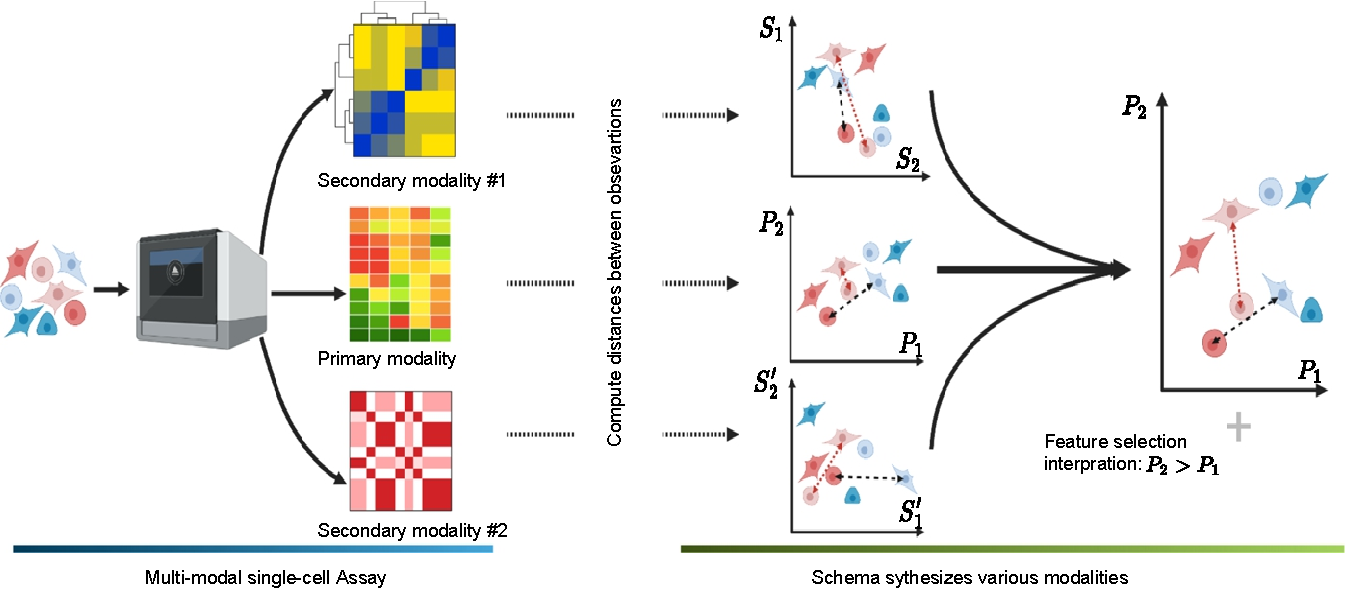
\includegraphics[width=0.8\textwidth]{Alg_Schema/fig}
  	\vspace{0.1cm}
  	\caption[Illustration of Schema integration competing method.]{\textbf{Illustration of Schema integration competing method.} Schema explores metrics learning to re-weigh modality features through maximizing the agreement with other modalities. Specifically, it utilizes quadratic programming~(QP) to learn a scaling transformation $u$ for the primary matrix $X$ such that pairwise distances of the transformation $u * x_i$~(where $*$ is coordinate-wise multiplication, for each $x_i\in X$) are highly correlated in other modalities. \emph{Source~\cite{singh2021schema}}~(modified to fit thesis format and/or clarify key points)
  }
  	\label{fig:Alg_Schema}
\end{figure} 

  \item[Schema]
  Schema~\citep{singh2021schema} applied metrics learning to reweigh modality features by maximizing the agreement with other modalities. Specifically, it utilizes quadratic programming~(QP) to learn a scaling transformation $u$ for the primary matrix $X$ such that pairwise distances of the transformation $u * x_i$~(where $*$ is coordinate-wise multiplication, for each $x_i\in X$) are highly correlated other modalities. Specifically, it assumes $N$ observations across $r$ datasets $D_j$, where $j=1,\cdots,r$ and $D_j = \{x_i^{j}: i = 1,2,\cdots,N\}$ contains data for each observation. First, it refers $D_1$ as the primary modality and $D_2,\cdots,D_r$ as the secondary modalities. Next, it computes the pairwise distances $\rho_1,\cdots,\rho_j$ for each modality $D_j$ where $\rho_j(x_n^{j}, x_m^{(j)})$ is the distance between observation $n$ and $m$ in $D_j$. Then, it aims to find a transformation $\Omega$ with $\Omega(D)$ generating a dataset $D^{*}$ such that the Euclidean metric $\rho^{*}$ on $D^{*}$ on $D^{*}$ aligns the various metrics. $\Omega$ is limited to be a scaling transformation $\Omega(D) = \{diag(u)x: x \in D\}$, where $u \in \mathbb{R}^{k}$ and $diag(u)$ is a $k\times k$ diagonal matrix with diagonal entries $u$. Then, the squared distance between points under the transformation is given by:
  \begin{equation}
  \rho^{*}(x_n, x_m) = \|diag(u)x_n - diag(u)x_m\|^2 = \|diag(w)(x_n - x_m)\|^2
  \end{equation}
  where $w$ is the element-wise square of u. The scaling transforms u acts as a feature-weighting mechanism to choose the features of $D_1$ that align the datasets best. Schema integrates between the metrics $\rho_j$ to learn a metric $\rho^{*}$ that aligns well with all of them. The correlation between $\rho^{*}$ and $\rho_j$ is measured by the Pearson correlation coefficient. And to tackle multiple modalities, Schema maximizes the sum of Pearson correlation between $\rho^{*}$ and all other modalities pairwise distances $\rho_2,\cdots,\rho_j$~(\fref{fig:Alg_Schema}).
\begin{figure}[!h]
  	\centering
  	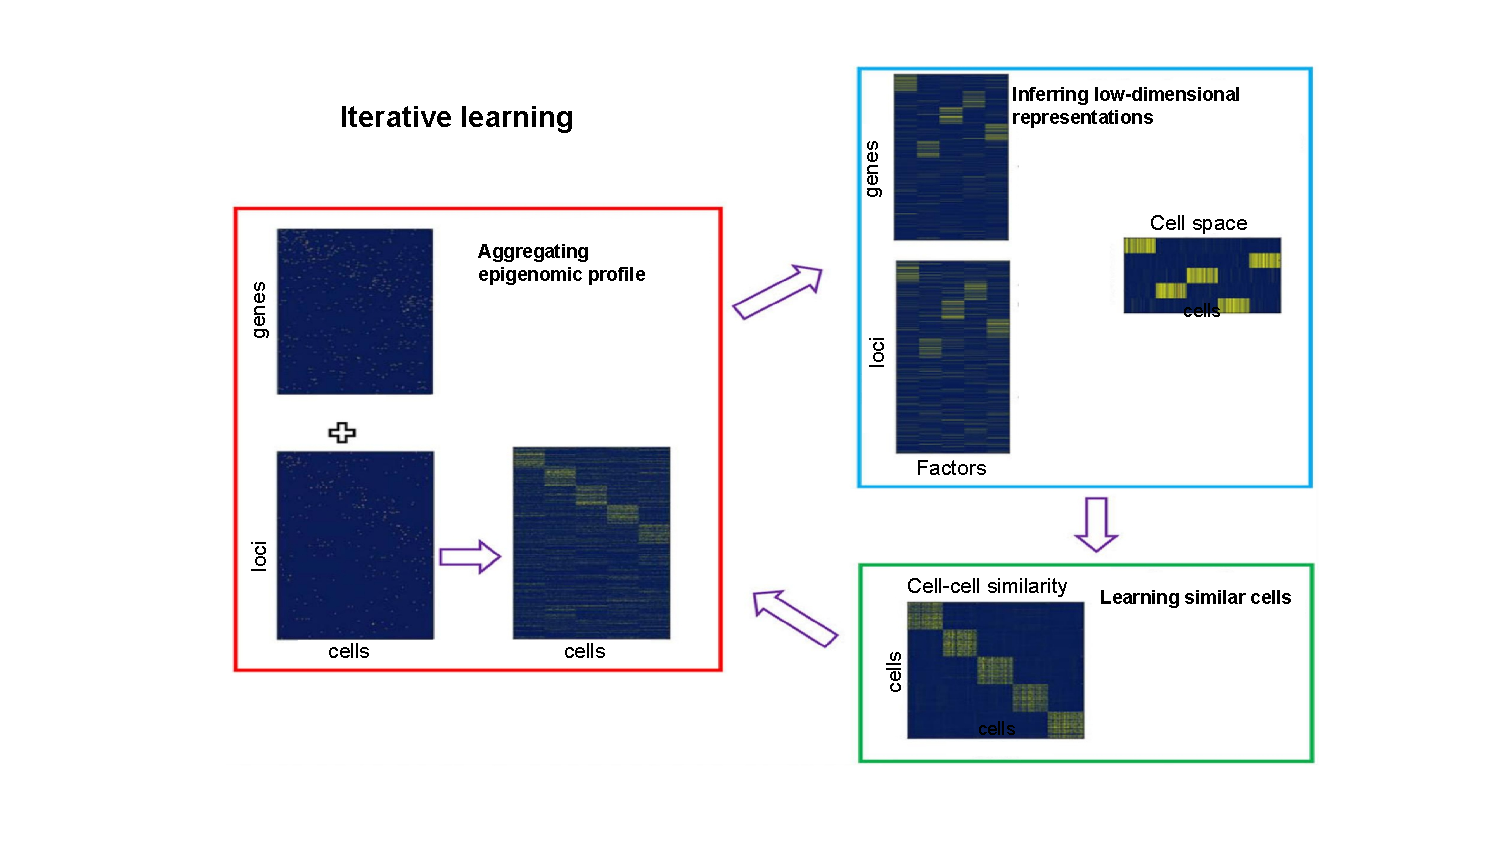
\includegraphics[width=0.55\textwidth]{Alg_scAI/fig}
  	\vspace{0.1cm}
  	\caption[Illustration of Seurat scAI integration competing method.]{\textbf{Illustration of Seurat scAI integration competing method.} scAI iteratively learns aggregated epigenomic profiles and low-dimensional representations from parallel scRNA-seq and scATAC-seq/single cell DNA methylation data. Input matrices consist of cells in rows and genes or loci in columns. The first step involves aggregating the epigenomic profile based on a randomly initiated cell-cell similarity matrix. In the second step, both transcriptomic and aggregated epigenomic data are concurrently decomposed into low-rank matrices, with gene, locus, and cell loading matrices indicating contributions for each factor. The third step computes a cell-cell similarity matrix based on the cell loading matrix. These steps iterate until a predefined stop criterion is met. \emph{Source~\cite{jin2020scai}}~(modified to fit thesis format and/or clarify key points)
  }
  	\label{fig:Alg_scAI}
\end{figure}

  \item[scAI]
  Single-cell Aggregation and Integration~(scAI)~\citep{jin2020scai} is aimed to integrate multiple modalities with different feature types specific for scRNA $(X_1\in \mathbb{R}^{p \textbf{ genes} \times n \textbf{ cells}})$ and scATAC/DNA methylation$(X_2\in \mathbb{R}^{q \textbf{ loci}\times n \textbf{ cells}})$ modalities. It creates a matrix factorization model:
  \begin{equation}
  \min_{w_1,W_2,H,Z\geq 0} \alpha \|X_1-W_1H\|_F^2 + \|X_2(Z \circ R)-W_2H\|_F^2 + \lambda \|Z-H^\top H\|_F^2 + \gamma\sum_j \|H_{.j}\|_1^2
  \end{equation}
  Where $W_1$ and $W_2$ are the gene loading and locus loading matrices with size $p\times K$ and $q\times K$($K$ is rank), respectively. Each of the $K$ columns is considered as a factor to capture a biological process/signal relating to a specific cell type. $W_1^{ik}$ and $W_2^{ik}$ are the loading values of gene $i$ and locus $i$ in factor $k$, and the loading values represent the contributions of gene $i$ and locus $i$ in factor k. $H$ is the cell loading matrix with size $K\times n$($H_{.j}$ is the $j$th column of $H$), and the entry $H^{kj}$ is the loading value of cell $j$ when mapped onto factor $k$. $Z$ is the cell-cell similarity matrix. $R$ is a binary matrix generated by a binomial distribution with a probability $s$. $\alpha, \lambda, \gamma$ are regularization parameters, and the symbol $\circ$ represents dot multiplication~(\fref{fig:Alg_scAI}).


\begin{figure}[!h]
  	\centering
  	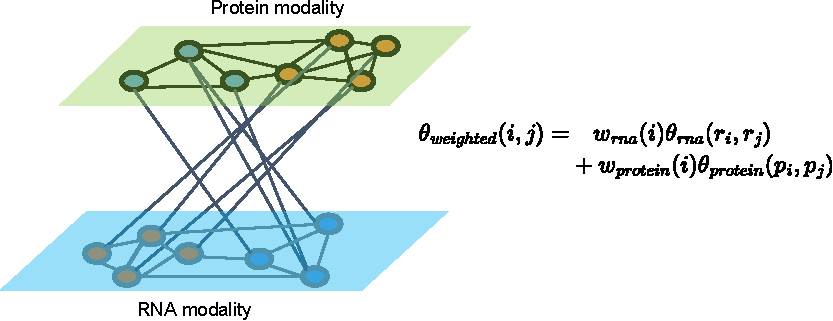
\includegraphics[width=0.60\textwidth]{Alg_WNN/fig}
  	\vspace{0.1cm}
  	\caption[Illustration of Seurat WNN integration competing method.]{\textbf{Illustration of Seurat WNN integration competing method.} Seurat weighted nearest neighbor(WNN) constructs a single unified representation across multiple modalities by initially creating k-nearest neighbor~(KNN) graphs for each modality based on the latent representation of each feature matrix. Subsequently, it calculates affinities using the exponential kernel between a cell and the average nearest neighbors for each modality. The latter is utilized to weigh cells in the unified representation. \emph{Source~\cite{hao2021seurat4}}~(modified to fit thesis format and/or clarify key points)
  }
  	\label{fig:Alg_WNN}
\end{figure}

  \item[Seurat WNN]
  Weighted nearest neighbor~(WNN)~\citep{hao2021seurat4}) constructs a single unified representation across multiple modalities. First, it creates k-nearest neighbor~(KNN) graphs for each modality based on the latent representation of each feature matrix. Next, it calculates affinities using the exponential kernel between a cell and the average NN for each modality. The latter is used to weigh cells. It finally calculated the weighted similarity between $cell_i$ and $cell_j$ as the dot product of $\textbf{w}_m(i)$ and $\theta(i,j)$,
  \begin{equation}
  	\theta_{weighted}(i,j)=\sum_{m} \textbf{w}_m(i)\theta(i,j)
  \end{equation}
  Where $\textbf{w}_m(i)$ is the weight of cell $i$ in modality $m$ and $\theta(i,j)$ denotes the affinity between cell $i$ and cell $j$ in modality $m$~(\fref{fig:Alg_WNN}).


  \item \textbf{Symphony Integration}
  Symphony~\citep{kang2021symphony} is a method to create single cell reference atlas for subsequent annotation of new single cell data sets. For a single case study with a multi-ome CITE-seq data, Symphony used canonical correlation analysis to find shared references. This simple procedure differs from MOJITOO in several ways: it does not use dimension reduction as input; it is not able to cope with more than 2 modalities and it uses the latent space of only one modality~(RNA) as shared space. Moreover, Symphony included the execution of batch correction with Harmony after the execution of CCA.

\end{description}


\subsubsection{Single Cell Multimodal Integration Objective}
Single-cell simultaneous modalities profiling is a nascent area, offering insights into biological processes and cellular heterogeneity. However, the complexity of different modalities' features and the growing library size present challenges, necessitating tools for integration In this thesis, we investigate the aspects with the flowing goals to develop a single cell multimodal integration method:

\begin{itemize}
	\item
	The objective is to develop an innovative computational method proficient in integrating more than two modalities with efficacy. The method should adeptly handle scenarios where modalities lack shared features and effectively address batch correction issues arising from diverse data batches. Furthermore, the method must yield a cohesive latent space suitable for clustering, data visualization, and subsequent analyses. Crucially, this latent space should be interpretable, facilitating the association of a component with the original feature count matrix. This interpretability enables a nuanced understanding of components, encompassing aspects such as gene expression and TF activity. Lastly, the methods should be computationally efficient to handle the increasingly larger single-cell library sizes.
	\item
	Establishing a comprehensive benchmarking framework for multimodal integration is imperative. All methods aferomentioned in \sref{background:sec2:integration} will be evaluated in \sref{chapter:MOJITOO_bench}. Acknowledging that ground truth labels~(cell type) may not infallibly represent actual biological facts due to manual cell annotation, it is crucial to devise a sophisticated set of benchmarking metrics. Beyond the clustering arrangement alignment with true labels, the benchmarking should encompass structural similarity evaluations between the shared latent space and each modality. Additionally, it should address the evolving levels of shared latent space distances among cells originating from the original modalities.

	\item
	We should curate diverse sets of simultaneous multimodal datasets for benchmarking, incorporating two datasets that simultaneously profile single-cell RNA sequencing~(scRNA) and single-cell Assay for Transposase-Accessible Chromatin sequencing~(scATAC), two datasets comprising scRNA and single-cell surface protein information, and two datasets involving all three prevalent types: scRNA, scATAC, and single cell surface protein. This comprehensive approach ensures a more equitable and robust benchmarking outcome.

	\item
	We should strive to interpret the components of the latent space using a dataset, gaining biological insights to determine whether it effectively captures cell type signals or signals related to cell fate differentiation. Additionally, we aim to interpret the latent space by associating it with the gene expression count matrix and epigenomic peak count matrix, selecting features to demonstrate the capabilities of our model.
\end{itemize}
\FloatBarrier %% step figure jump to the next subsection.

\subsection{Single Cell Multimodal Trajectory Inference}
We will present the computational challenge of trajectory inference for single-cell multimodal data, provide an overview of current methods developed in this field, and outline our goals to develop a method that addresses these challenges.

\subsubsection{Challenge of Single Cell Trajectory Inference}
\label{background:sec2:challenge_TI}
Computational trajectory analysis, which explores non-linear embeddings in the cellular space and algorithms to find paths or trees in these spaces, is quite popular in the analysis of single cells~\citep{wolf2019paga,chen2019stream,street2018slingshot,Lynch2022}. Despite the power of these approaches~\citep{saelens2019comparison}. There are still some challenges that need to be addressed:

\begin{figure}[!h]
	\centering
	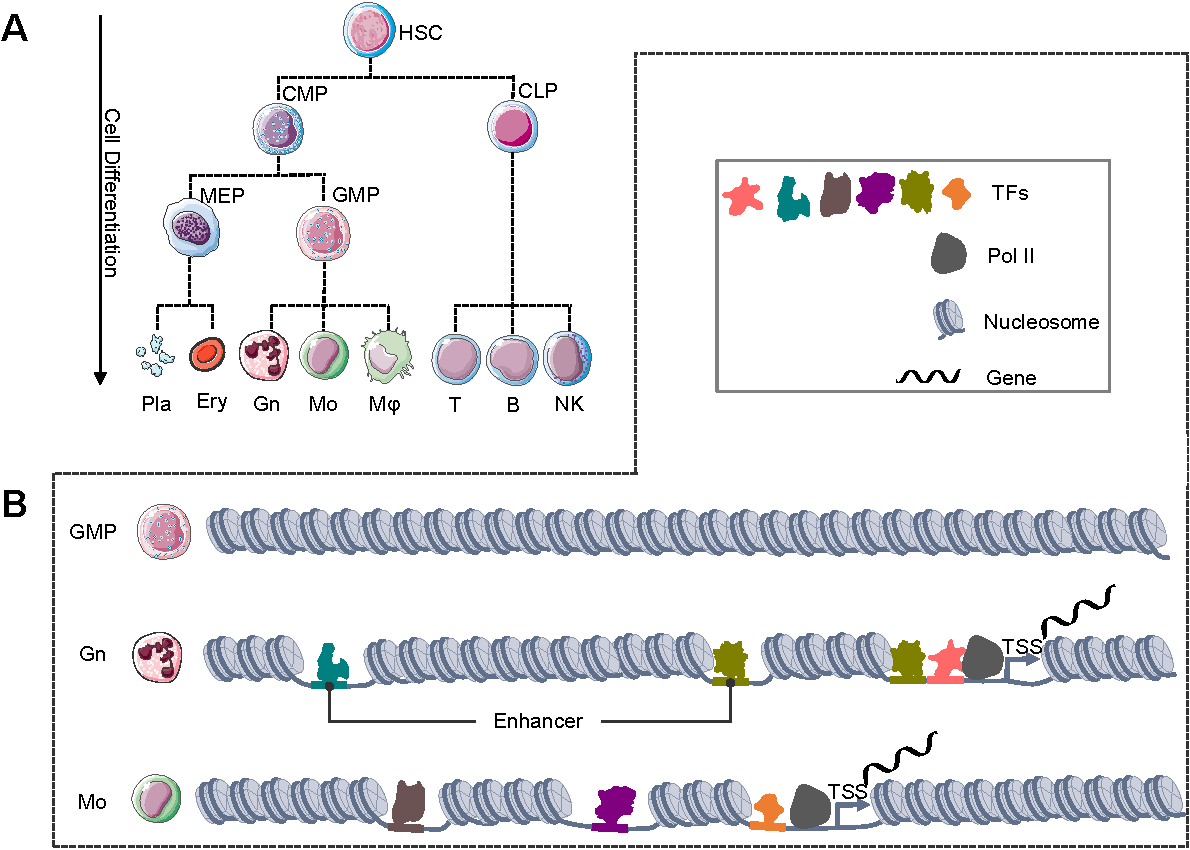
\includegraphics[width=0.95\textwidth]{cell_differentiation/fig}
	\vspace{0.1cm}
	\caption[Hematopoiesis Cellular Differentiation]{\textbf{Hematopoiesis Cellular differentiation.} \textbf{A)} Hematopoiesis differentiation tree. Cell types are hematopoietic stem cell~(HSC), common myeloid progenitor~(CMP),  common lymphoid progenitor~(CLP), megakaryocyte–erythroid progenitor cell~(MEP), granulocyte-macrophage progenitor~(GMP), platelet~(Pla), erythrocyte~(Ery), granulocyte~(Gn), monocytes~(Mo), macrophages(M$\phi$), T cell~(T), B cell~(B) and Natural killer cell~(NK). \textbf{B)} GMP differentiation into two cell types~(Gn and Mo). GMP cells undergo differentiation into two distinct cell types, namely, granulocytes~(Gn) and monocytes~(Mo). During this differentiation process, specific regions of the chromatin become open, and different transcription factors bind to these regions, ultimately influencing the gene expression patterns that characterize these two cell types. \emph{Source:~\cite{costa2023dissecting}}~(modified to fit thesis format and/or clarify key points)}
	\label{fig:cell_differentiation}
\end{figure}

\begin{itemize}
	\item \textbf{Cell Differentiation in Biology:}
	The cell types in a multicellular organism become different from one another, as illustrated in \fref{fig:cell_differentiation}A, which shows a hematopoiesis differentiation tree. This cellular differentiation process is controlled by transcription factors~(TFs) binding to specific DNA regions called enhancers/promoters to recruit polymerases and modulate the expression of genes, eventually leading to the formation of different cell types~(\fref{fig:cell_differentiation}B)~\citep{costa2023dissecting}. Multimodal data with simultaneous epigenome and transcriptome information provide a better opportunity to explore this process. However, few trajectory inference methods make use of multimodal data to inspect cellular differentiation events.


	\item \textbf{Complexity of multi-branching trajectories:}
	For complex datasets, such as hematopoiesis(~\fref{fig:cell_differentiation}A), where cell differentiation leads to various immune cell types, monocytes, myeloid cells, and their subtypes, a method capable of capturing intricate differentiation processes is required. Unfortunately, many existing methods struggle to accurately capture the trajectory structure of such complex datasets.


	\item \textbf{Most approaches use low number of dimensions($\geq3$) to fit trajectories:}
	As high-dimensional data cannot be naturally visualized, trajectories of single-cell data are typically represented in embeddings with only 2 to 3 dimensions. However, this approach necessitates the omission of high-dimensional information. To address this limitation, there is a need for methods that directly infer cell differentiation from high-dimensional embeddings.

	\item \textbf{Graph-based methods only use the information of nodes:}
	Methods such as Minimum Spanning Tree, ElPiGraph, or diffusion processes typically focus solely on cell position information, capturing only the relation between cells. These approaches neglect high-order graph features such as edges and triangles, which grasp the relationship between edges and triangles.

	\item \textbf{Few Methods are designed for multimodal data:}
	In the emerging field of single-cell multimodal analysis, many methods lack a comprehensive approach to trajectory inference across multiple modalities. While existing methods designed for single-cell transcriptomics, such as Slingshot and STREAM, can be applied to handle single-cell multimodal data, they often fall short in leveraging multimodal information for in-depth analyses, such as exploring gene regulation along a trajectory path using information from multiple modalities.
\end{itemize}
% a figure shows the feature type differences among different modalities

% a figure of single cell multimodal integration methods theory
\label{background:sec2:TI}
\subsubsection{Computational Methods for Trajectory Inference}
 The challenges highlighted in \sref{background:sec2:challenge_TI} regarding the trajectory inference of single-cell multimodal data present complexities in developing methods for handling multimodal data and data exhibiting intricate trajectory structures.

% table summarizing method
\begin{table}[!ht]
	\small
	\centering
	\begin{tabular}{llll}
		\toprule
		Name & Programming & Technique & Reference \\
		\midrule
    Celltree& R& LDA & \cite{duverle2016celltree}\\
    ElPigraph& Python/R & ElPigraph & \cite{albergante2020ElPiGraph}\\
    Monocle3 & R  & DDRTree/SimplePPT/L1Graph  & \cite{cao2019monocle3} \\
    MST & R & MST &  \cite{book2023mclust}\\
    PAGA	 & Python & kNN graph partitioning & \cite{wolf2019paga} \\
    pCreode & Python & d-kNN graph & \cite{herring2018pCreode} \\
		RaceID/StemID &  R & k-medoids clustering &  \cite{grun2016stemid} \\
    SLICE& R & MST & \cite{guo2017slice}\\
		Slingshot & R & MST & \cite{street2018slingshot}\\
		STREAM& Python & ElPigraph & \cite{chen2019stream}\\
    TSCAN & R & MST &  \cite{ji2016tscan}\\
		\bottomrule
	\end{tabular}
	\vspace{0.1cm}
	\caption[Overview of computational trajectory inference methods]{Overview of computational trajectory inference methods.}
	\label{tab:methods_ti_overview}
\end{table}
Next, we will discuss several published trajectory inference methods, All of them are top methods according to the dynverse trajectory inference evaluation system~\citep{saelens2019comparison} except STREAM a new method not yet implemented in dynverse. These methods can be broadly categorized into six groups. The first group involves methods utilizing a minimum spanning tree~(MST) to capture the backbone in the embeddings of a dataset~(e.g., TSCAN, slingshot, MST, slice). The second group includes methods like ElPiGraph, which leverages Elastic Principal Graphs to yield an explicit principal tree in data space~(ElPiGraph, STREAM). The third group employs topic model Latent Dirichlet Allocation~(LDA) from the natural language processing~(NLP) field for inference. The fourth group encompasses methods such as PAGA, using kNN graph partitioning, and pCreode, creating a d-kNN graph. The fifth group utilizes cluster distances for inference to derive the structure~(RaceID/StemID). The last method, Monocle3, seeks to create a principal graph on dimension reductions. These methods are summarized in \tref{tab:methods_ti_overview} illustrates the workflow of most of the methods.
\begin{description}

\begin{figure}[h!]
  	\centering
  	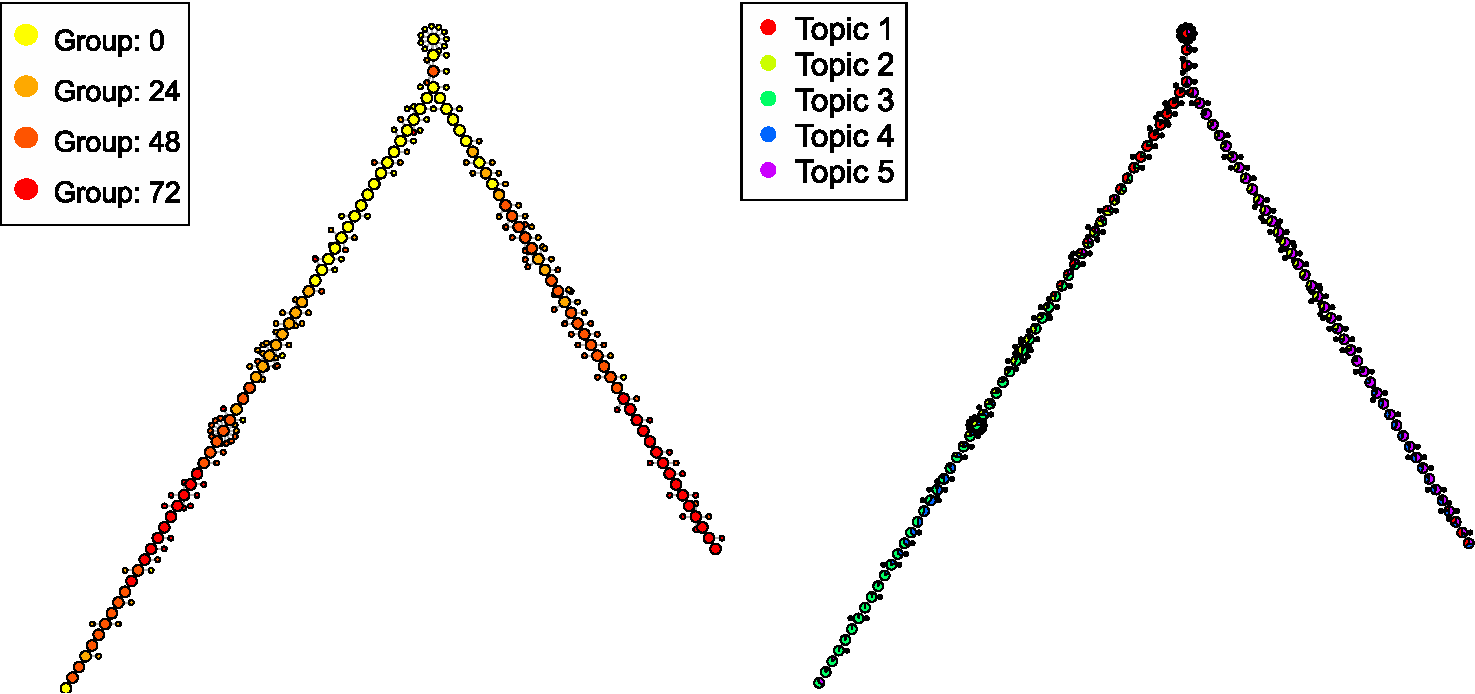
\includegraphics[width=0.55\textwidth]{TI_Alg_celltree/fig}
  	\vspace{0.1cm}
  	\caption[Illustration of TI method Celltree schematic.]{\textbf{Illustration of TI method Celltree schematic.} Celltree use myoblast data as example. Backbone tree obtained from the dataset of differentiating myoblasts with cellTree. Larger nodes indicate backbone cells~(selected representatives), whereas smaller nodes represent cells that only show slight variations from the backbone cell they are attached to. Cell nodes have been coloured according to \textbf{A} their sampling time~(in hours from the start of the differentiation process) and \textbf{B} their distribution over topics. \emph{Source:~\cite{duverle2016celltree}}~(modified to fit thesis format and/or clarify key points)
  	}
  	\label{fig:TI_Alg_celltree}
\end{figure}
  \item[Celltree]
  To identify and utilize group structure, Celltree~\citep{duverle2016celltree} adapts a natural language processing~(NLP) statistical approach known as Latent Dirichlet Allocation~(LDA) to build a topic model. By comparing the different per-cell topic histograms, celltree can evaluate their similarity and infer complex hierarchical structures. By looking at the topics themselves, one can obtain useful biological insights into the gene sets characterizing the different stages of that hierarchy. Based on this lower-dimensional model, it constructs a visual representation of the cell population. finally, Celltree introduces ``backbone trees'' to easily visualize cells along complex differentiation paths~(\fref{fig:TI_Alg_celltree}).
  

\begin{figure}[h!]
  	\centering
  	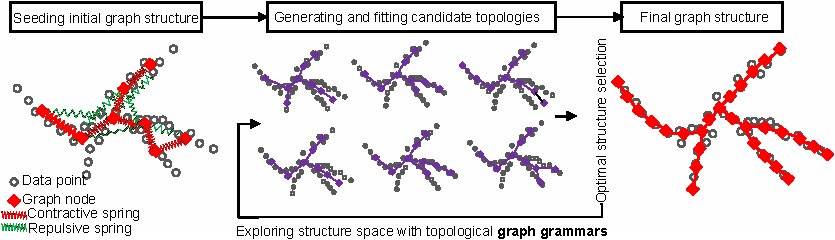
\includegraphics[width=0.85\textwidth]{TI_Alg_ElPiGraph/fig}
  	\vspace{0.1cm}
  	\caption[Illustration of TI method ElPiGraph schematic.]{\textbf{Illustration of TI method ElPiGraph schematic.} Schematic workflow of the ElPiGraph method. On the left, the construction of the elastic graph starts by defining the initial graph topology and embedding it into the data space. The graph structure is fitted to the data, minimizing the mean square error regularized by the elastic energy. The elastic energy includes a term reflecting the overall stretching of the graph~(symbolically shown as contractive red springs) and a term reflecting the overall bending of the graph branches and the harmonicity of branching points~(shown as repulsive green springs). In the middle, ElPiGraph explores a large region of the structural space by exhaustively applying a set of graph rewriting rules~(graph grammars) and selecting, at each step, the structure leading to the minimum overall energy of the graph embedding. \emph{Source:~\cite{cao2019monocle3}}~(modified to fit thesis format and/or clarify key points)
  	}
  	\label{fig:TI_Alg_ElPiGraph}
\end{figure}

  \item[ElPiGraph]
  Elastic Principal Graphs~(ElPiGraphs)~\citep{albergante2020ElPiGraph} serve as structured approximators for data, comprising vertices connected by edges. These vertices are embedded into the data space, minimizing mean squared distance~(MSD) to data points. Notably, ElPiGraphs differ from unstructured k-means by incorporating edges to define an elastic energy term. This term, coupled with MSD, penalizes edge stretching and branch bending. ElPiGraph employs a topological grammar for optimal graph structure determination, building on a core algorithm initially introduced and tested in earlier publications~\citep{gorban2007topological}. In essence, an elastic principal graph is an undirected graph in multidimensional space, optimizing data approximation and graph elastic energy. Key parameters, including trimming radius~($R_0$), edge elasticity~($\lambda$), star bending elasticity~($\mu$), and a complexity control coefficient~($\alpha$), guide the optimization process. ElPiGraph achieves efficient minimization by employing a quadratic problem-solving approach for vertex coordinates. It uses topological grammars, exploring diverse graph structures, and iteratively refining configurations until specified conditions are met. Finally, ElPiGraph yields an explicit principal tree in data space, facilitating independent study or mapping data onto the tree for analysis in intrinsic coordinates~(\fref{fig:TI_Alg_ElPiGraph}).


\begin{figure}[h!]
  	\centering
  	\includegraphics[width=0.90\textwidth]{TI_Alg_Monocle3/fig}
  	\vspace{0.1cm}
  	\caption[Illustration of TI method Monocle3 schematic.]{\textbf{Illustration of TI method Monocle3 schematic.} Monocle3 aims to learn a principal graph by using SimplePPT, DDRTree or L1Graph, with which, each cell is projected onto the graph. By selecting the starting points on the graph, Monocle measures the distance from these points to each cell, determining a cell's pseudotime as the distance to the closest starting point on the graph. \emph{Source:~\cite{cao2019monocle3}}~(modified to fit thesis format and/or clarify key points)
  	}
  	\label{fig:TI_Alg_Monocle3}
\end{figure}

  \item[Monocle3]
  Monocle3 undergoes a comprehensive five-step process in single-cell dataset analysis~\citep{cao2019monocle3}. Firstly, it normalizes and pre-processes data, addressing technical variations. The second step involves reducing dimensionality by projecting cells onto the top 50 principal components, with options for further reduction using t-SNE or UMAP. In the third step, Monocle 3 clusters and partitions cells, recognizing disconnected trajectories or ``supergroups" that capture diverse cellular responses. Subsequently, it learns a principal graph, utilizing methods like DDRTree, SimplePPT, or L1Graph, accommodating tree-like or looped trajectories. Finally, Monocle 3 conducts differential expression analysis and visualization for exploring gene dynamics across clusters and trajectories with sophisticated testing methods~(\fref{fig:TI_Alg_Monocle3}).

\begin{figure}[h!]
  	\centering
  	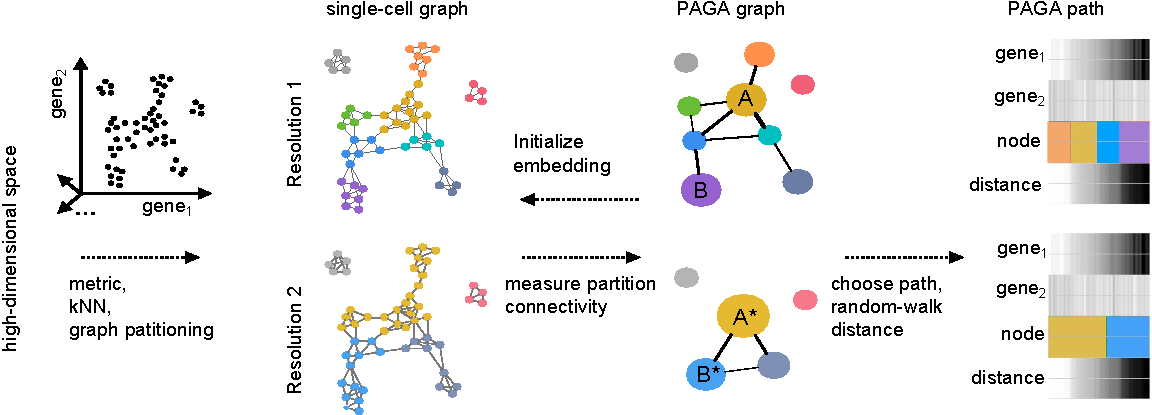
\includegraphics[width=0.85\textwidth]{TI_Alg_PAGA/fig}
  	\vspace{0.1cm}
  	\caption[Illustration of TI method PAGA schematic.]{\textbf{Illustration of TI method PAGA schematic.}
  	PAGA uses partition-based graph abstraction generating a topology-preserving map of single cells. It creates a kNN graph and partitions it using the Louvain algorithm at a desired resolution where partitions represent groups of connected cells. Next, A PAGA graph is obtained by associating a node with each partition and connecting each node by weighted edges that represent a statistical measure of connectivity between partitions. PAGA graphs reveal the denoised topology of the data at a chosen resolution by discarding low-weight edges. \emph{Source:~\cite{wolf2019paga}}~(modified to fit thesis format and/or clarify key points)
  	}
  	\label{fig:TI_Alg_PAGA}
\end{figure}

  \item[PAGA]
  Probabilistic Approximate Graph Abstraction~(PAGA) uses partition-based graph abstraction generating a topology-preserving map of single cells~\citep{wolf2019paga}. High-dimensional gene expression data is represented as a kNN graph by choosing a suitable low-dimensional representation and an associated distance metric for computing neighborhood relations. The kNN graph is partitioned using the Louvain algorithm at a desired resolution where partitions represent groups of connected cells. A PAGA graph is obtained by associating a node with each partition and connecting each node by weighted edges that represent a statistical measure of connectivity between partitions. By discarding spurious edges with low weights, PAGA graphs reveal the denoised topology of the data at a chosen resolution and reveal its connected and disconnected regions. Combining high-confidence paths in the PAGA graph with a random-walk-based distance measure on the single-cell graph, PAGA orders cells within each partition according to their distance from a root cell. A PAGA path then averages all single-cell paths that pass through the corresponding groups of cells. This allows to trace gene expression changes along complex trajectories at single-cell resolution~(\fref{fig:TI_Alg_PAGA}).

\begin{figure}[h!]
  	\centering
  	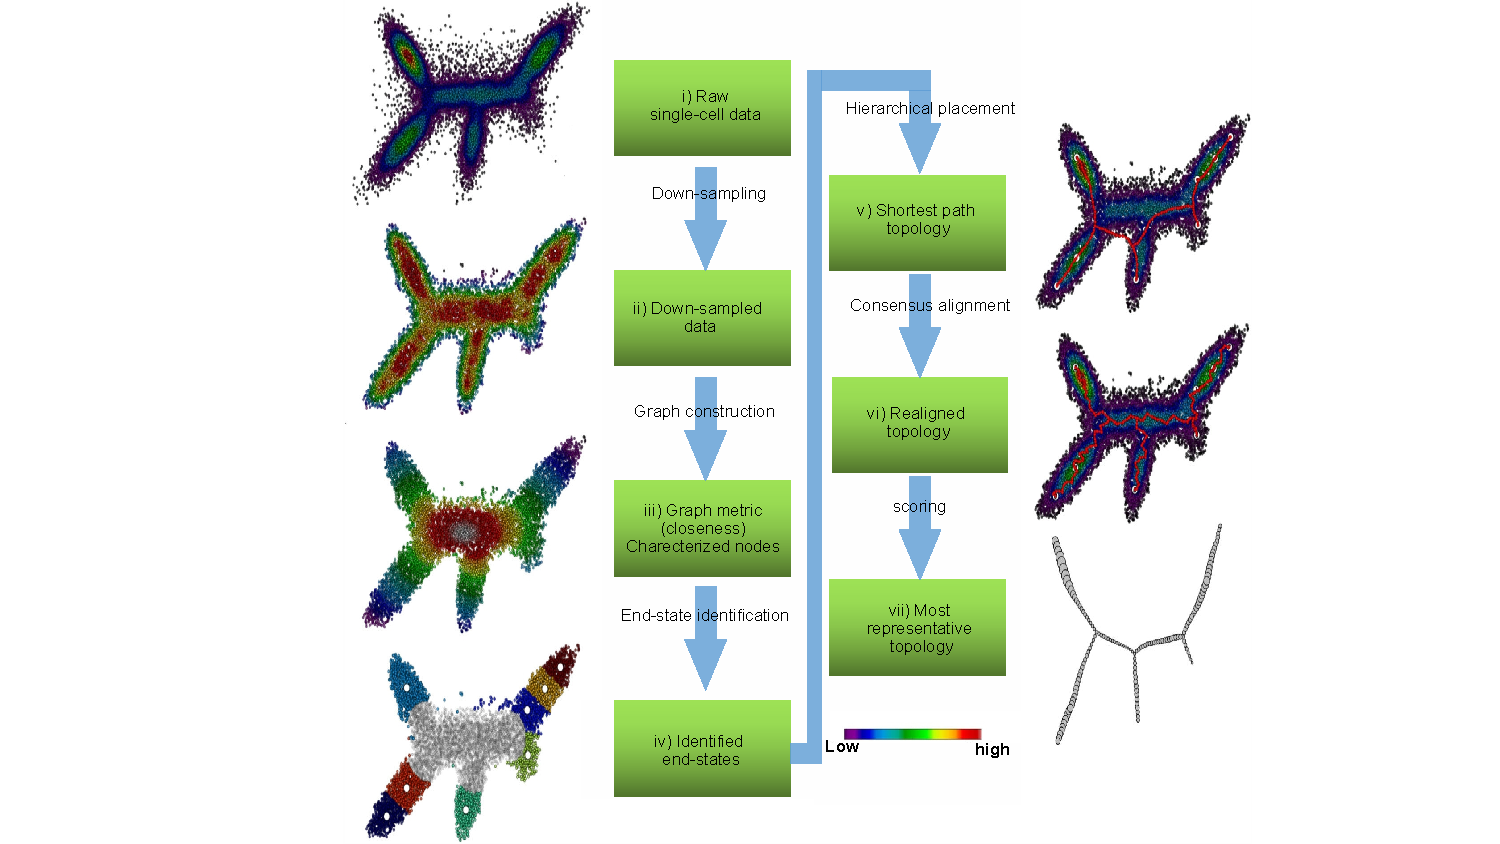
\includegraphics[width=0.65\textwidth]{TI_Alg_pCreode/fig}
  	\vspace{0.1cm}
  	\caption[Illustration of TI method pCreode schematic.]{\textbf{Illustration of TI method pCreode schematic.} pCreode carries out 6 steps to infer a trajectory. It creates a density-based k-nearest neighbor~(d-kNN) network and constructs topology with a hierarchical placement strategy of cells on path nodes between end-state clusters. Next, it iteratively redoes the arrangement of the topology according to the neighborhood cell densities. \emph{Source:~\cite{herring2018pCreode}}~(modified to fit thesis format and/or clarify key points)
  	}
  	\label{fig:TI_Alg_pCreode}
\end{figure}

  \item[pCreode]
  %pCreode infer a trajactory for single-cell data through 7 steps:~(i) Input single-cell expression data.~(ii) Density-normalized representation after down-sampling the original dataset. Overlay shows density post down-sampling.~(iii) Density-based k-nearest neighbor~(d-kNN) network from down-sampled data. Overlay represents closeness centrality, a surrogate for cell state.~(iv) K-means clustering identifies end-states based on low closeness values~($<$mean). The number of clusters is doubled for rare cell types.~(v) Topology constructed with a hierarchical placement strategy between end-states, allowing data points along an ancestral continuum. Overlay shows original cell density.~(vi) Aligned topology~(red) achieved through iterative assignment and repositioning of path nodes using neighborhood cell densities.~(vii) Representative topology extracted using p-Creode scoring from an ensemble of N topologies, with node size indicating the original cell density.

  pCreode infer a trajactory for single-cell data through 6 steps~\citep{herring2018pCreode}. 1) Conducts density-dependent down-sampling to normalize the representation of both rare and overrepresented cell states; 2) Constructs a density-based k-nearest neighbor~(d-kNN) network using the down-sampled data; 3) Automatically distinguishes end-states from transition states by employing K-means clustering and assessing silhouette scores for cells with low closeness values~(< mean); 4) Establishes topology through a hierarchical placement strategy, positioning cells on path nodes between end-states; 5) Aligns topology with maximal consensus through an iterative process involving the assignment and repositioning of path nodes based on neighborhood cell densities; 6) Develops a scoring metric within pCreode to compare dissimilarities between topologies facilitating the selection of the most representative graph for visualization purposes~(\fref{fig:TI_Alg_pCreode}).

  \begin{figure}[h!]
  	\centering
  	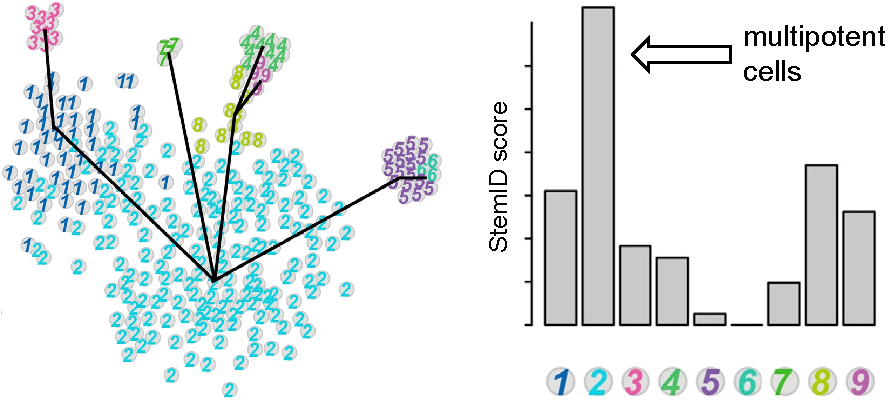
\includegraphics[width=0.55\textwidth]{TI_Alg_StemID/fig}
  	\vspace{0.1cm}
  	\caption[Illustration of TI method RaceID/StemID schematic.]{\textbf{Illustration of TI method RaceID/StemID schematic.}
  	RaceID/StemID initially conducts clustering using RaceID2~(k-medoids clustering). Next, it infers putative differentiation trajectories by linking the medoids of two clusters, defining the possible topology of the lineage tree. It then assigns each cell to an inter-cluster link by selecting the longest projection. \emph{Source:~\cite{albergante2020ElPiGraph}}~(modified to fit thesis format and/or clarify key points)
  	}
  	\label{fig:TI_Alg_StemID}
  \end{figure}

  \item[RaceID/StemID]
  StemID~\citep{grun2016stemid} uses RaceID~\citep{grun2015raceid}, an advanced version of RaceID to perform clustering. Next, to address the challenge of determining branching points in systems with multiple cell lineages for building the lineage tree with guided topology StemID predefines the tree's structure by allowing potential differentiation trajectories between pairs of clusters. Each trajectory links the medoids of two clusters, and collectively, these inter-cluster links determine the possible lineage tree's topology. To mitigate technical noise and computational load, It initially reduces input space dimensionality, emphasizing maximal preservation of point-to-point distances. Next, it assigns each cell to its likely position on a single inter-cluster link based on the projection of the vector connecting a cluster's medoid to one of its cells onto links with other clusters' medoids. By normalizing link lengths and identifying densely populated links, StemID discerns potential differentiation trajectories~(\fref{fig:TI_Alg_StemID}).

\begin{figure}[h!]
  	\centering
  	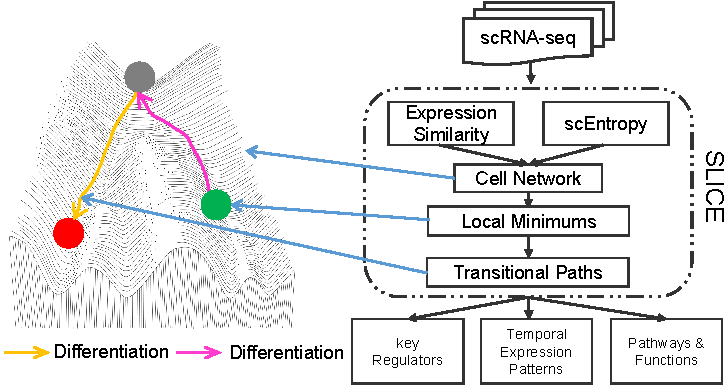
\includegraphics[width=0.65\textwidth]{TI_Alg_SLICE/fig}
  	\vspace{0.1cm}
  	\caption[Illustration of TI method SLICE schematic.]{\textbf{Illustration of TI method SLICE schematic.}
  	SLICE first measures cell differentiation states based on the calculation of single-cell entropy (scEntropy) and then predicts cell differentiation trajectories by ordering single cells according to their scEntropy-derived differentiation states. \emph{Source:~\cite{guo2017slice}}~(modified to fit thesis format and/or clarify key points)
  	}
  	\label{fig:TI_Alg_SLICE}
\end{figure}

  \item[SLICE]
  Single Cell Lineage Inference Using Cell Expression Similarity and Entropy~(SLICE)~\citep{guo2017slice} comprises two main functions: quantitatively assessing cell differentiation state through single-cell entropy and reconstructing single-cell lineages in silico. The calculation of single-cell entropy~(scEntropy) involves computing the expected value for each cell, representing the uncertainty in cellular functions activation based on gene expression patterns. The scEntropy is utilized to measure the differentiation state of individual cells. Stable states are identified within scRNA-seq datasets using clustering or graph-based methods, considering the scEntropy of each cell. SLICE then constructs a lineage model by inferring a directed minimum spanning tree among stable states, reflecting differentiation trajectories. The reconstruction of cell transitional paths involves either a shortest-path approach or a principal curve-based approach, revealing the dynamics of gene expression during differentiation. Lineage-dependent differentially expressed genes are identified based on smoothed expression profiles, and temporal gene expression patterns are unveiled through clustering analysis~(\fref{fig:TI_Alg_SLICE}).

\begin{figure}[h!]
  	\centering
  	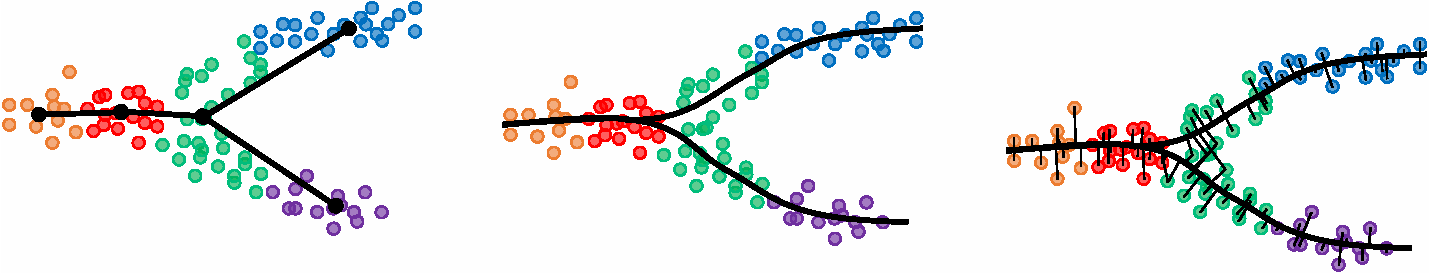
\includegraphics[width=0.8\textwidth]{TI_Alg_slingshot/fig}
  	\vspace{0.1cm}
  	\caption[Illustration of TI method Slingshot schematic.]{\textbf{illustration of TI method Slingshot schematic.}
  	Firstly, a Minimum Spanning Tree~(MST) is constructed on the clusters to determine the number and rough shape of lineages. Following that, simultaneous principal curves are employed to obtain smooth representations of each lineage. \emph{Source:~\cite{street2018slingshot}}~(modified to fit thesis format and/or clarify key points)
  	}
  	\label{fig:TI_Alg_slingshot}
\end{figure}

  \item[Slingshot]
  Slingshot~\citep{street2018slingshot} infers a trajectory of datasets with multiple branches by comprising two distinct stages: 1) Global Lineage Structure Inference. In this stage slingshot employs Minimum Spanning Tree~(MST) on clustered data points to infer the overall lineage structure. By utilizing a cluster-based MST, Slingshot stably identifies essential elements such as the number of lineages and their branching points. 2) Pseudotime Inference for Individual Lineages. In the second stage, Slingshot introduces a novel approach known as simultaneous principal curves. This method fittingly applies smooth branching curves to the identified lineages, translating the knowledge of the global lineage structure into reliable estimates of cell-level pseudotime variables for each lineage~(\fref{fig:TI_Alg_slingshot}).

\begin{figure}[h!]
  	\centering
  	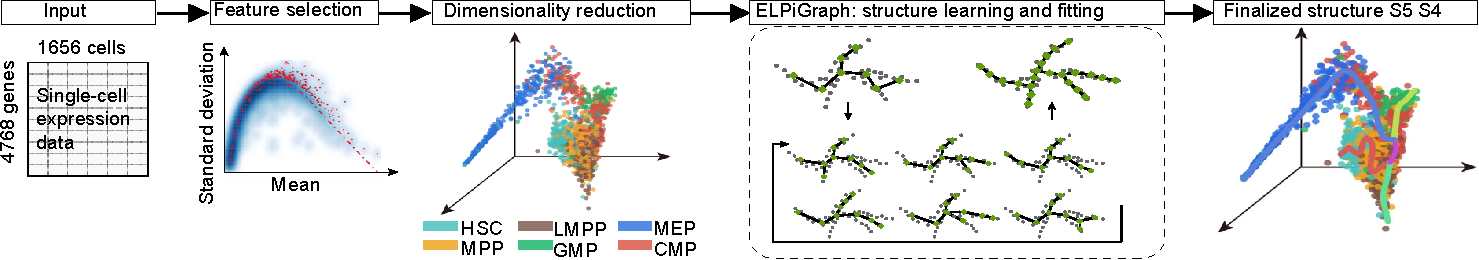
\includegraphics[width=0.95\textwidth]{TI_Alg_STREAM/fig}
  	\vspace{0.1cm}
  	\caption[Illustration of TI method STREAM schematic.]{\textbf{Illustration of TI method STREAM schematic.} STREAM first selection of informative genes from a single cell count matrix, followed by dimensional reduction. Next, it learns and fits simultaneous tree structure by ElPiGraph. The optimal structure is selected based on the elastic energy minimization among a set of candidate structures that are constructed every time a tree node is added. The final tree is interpreted as a set of connected curves representing different trajectories. \emph{Source:~\cite{chen2019stream}}~(modified to fit thesis format and/or clarify key points)
  	}
  	\label{fig:TI_Alg_STREAM}
\end{figure}

  \item[STREAM]
  Single-cell Trajectories Reconstruction, Exploration And Mapping~(STREAM) takes a single-cell gene expression matrix as input~\citep{chen2019stream}. Next, it performs three main steps: selection of informative genes, dimensionality reduction, and simultaneous tree structure learning and fitting by ElPiGraph. The optimal structure is selected based on the elastic energy minimization among a set of candidate structures that are constructed every time a tree node is added. The final tree is interpreted as a set of connected curves representing different trajectories~(\fref{fig:TI_Alg_STREAM}).

\begin{figure}[h!]
  	\centering
  	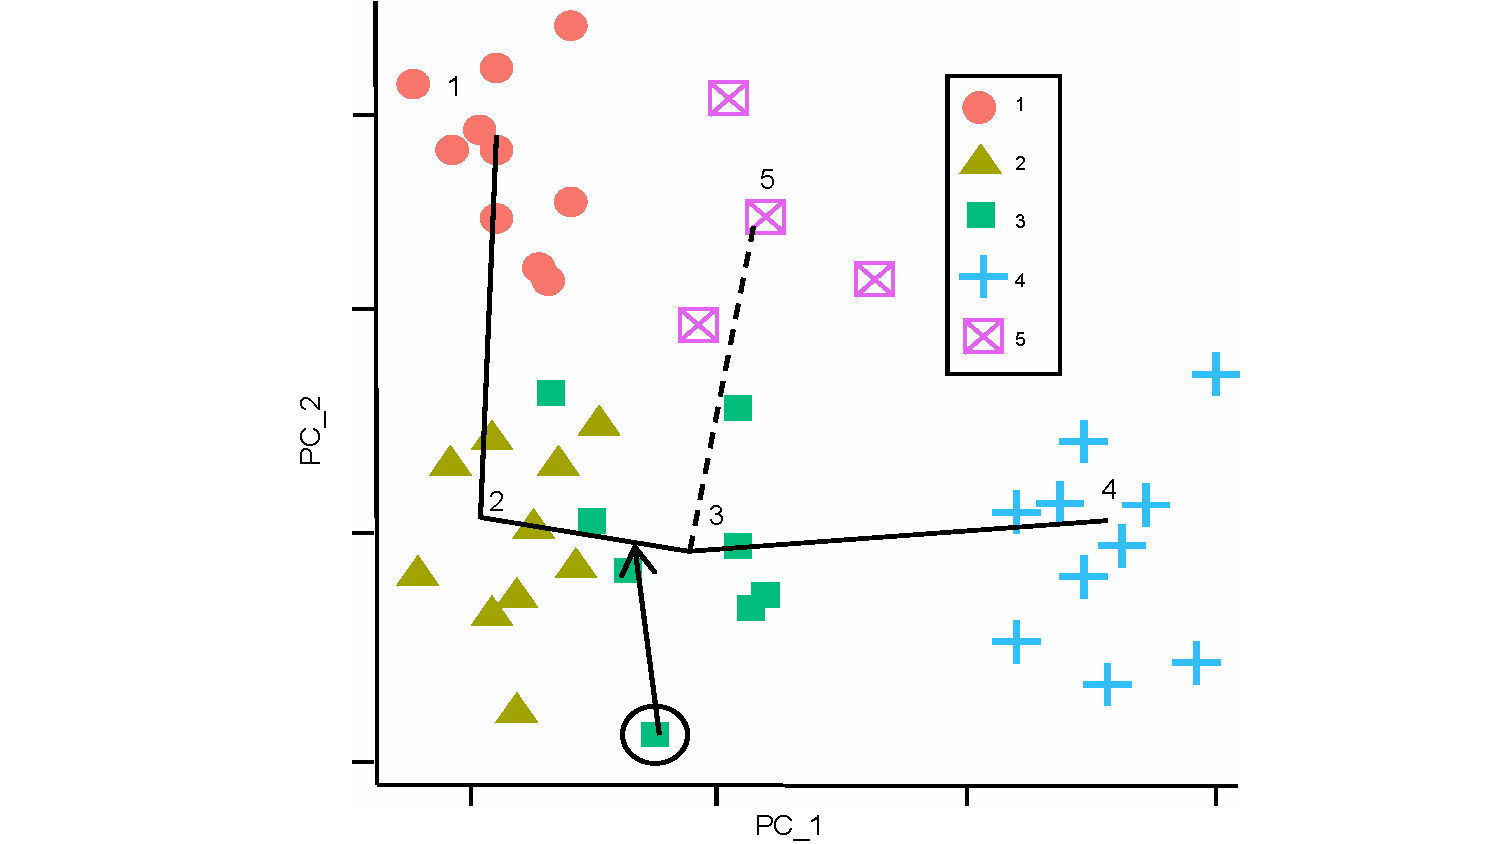
\includegraphics[width=0.65\textwidth]{TI_Alg_TSCAN/fig}
  	\vspace{0.1cm}
  	\caption[Illustration of TI method TSCAN schematic.]{\textbf{Illustration of TI method TSCAN schematic.}
  	TSCAN initially constructs a cluster-based Minimum Spanning Tree~(MST) with multiple paths. Next, TSCAN orders cells along each path by projecting them onto the tree edges. \emph{Source:~\cite{ji2016tscan}}~(modified to fit thesis format and/or clarify key points)
  	}
  	\label{fig:TI_Alg_TSCAN}
\end{figure}

  \item[TSCAN]
  pseudo-Time reconstruction in Single-Cell RNA-seq ANalysis~(TSCAN)~\citep{ji2016tscan} first uses PCA to reduce the dimensionality. It uses the clustering algorithm Mclust to model the datasets as a mixture of normal distributions, to cluster the cells while automatically determining the number of clusters using the Bayesian information criterion. Next, It infers a trajectory by identifying the longest connected path through the Minimum Spanning Tree~(MST) tree, which is created through the cluster center. Finally, all the cells are projected to the nearest point on the trajectory, creating the final ordering. TSCAN automatically determines both start and end cell clusters without prior gene dimension filtering. However, slight changes in center locations can significantly impact the identified trajectory~(\fref{fig:TI_Alg_TSCAN}).


\end{description}

%\subsubsection{Celltree}
%\subsubsection{ElPiGraph}
%\subsubsection{Monocle3}
%\subsubsection{PAGA}
%\subsubsection{pCreode}
%\subsubsection{RaceID/StemID}
%\subsubsection{SLICE}
%\subsubsection{Slingshot}
%\subsubsection{STREAM}
%The Elastic principal graph:
%\begin{equation}
%	\begin{aligned}
%& U^{\phi}(X, G) = \frac{1}{|x|}\sum_{j=1}^{|V|} \sum_{i:P(i)=j} \min \left(\left\|X_i - \phi(V_j)^2, R_0^2\right\|\right) \\
%&\quad + \sum_{E^{(i)}}[\lambda + \alpha(\max(2, \deg(E^{(i)}(0))) - 2)](\phi(E^{(i)}(0)) - \phi(E^{(i)}(1)))^2 \\
%&\quad + \mu \sum_{S^{(j)}} \left(\phi(S^{(j)(0)}) - \frac{1}{\deg (S^{(j)(0)})} \sum_{i = 1}^{\deg (S^{(j)(0)})}\right)^2
%	\end{aligned}
%\end{equation}
%where $X=\{X_i\}, i = 1\cdots|X|$ is a set of points, $E^{(i)}(0)$ and $E^{(i)(1)}$ denotes the two vertices of a graph edge $E^{(i)}$, and $S^{(j)(0)},\cdots S^{(j)}(k)$ denote the vertices of the a star $S^{(j)}$ in the graph. $P(i)$ is a data point partitioning function associating each data point $X_i$ to the closest vertex index that $P(i) = \arg\min_{j=1\cdots |V|}$. $phi{V_j}$ is the mapping function that $\phi: V \rightarrow R^{m}$, which defines a position of $j$th graph vertex in the multidimensional space of data. Finally, $R_0$ is the trimming radius such that points further than $R_0$ from any nodes don't contribute to the optimization of the graph, and $\lambda$ is the edge stretching elasticity modulo regularizing the total length of the graph, and $\alpha$ is a coefficient to control the complexity of the graph. $\mu$ is the star bending elasticity that controls the smoothness of the graph.
%\subsubsection{TSCAN}
%\subsubsection{Slicer}
%Slicer is a KNN-based trajectory inference method that utilizes alpha-hull to estimate the k parameter for locally linear embedding dimensionality reduction. First, Slicer computes a KNN graph from locally linear embedding, next it finds the most “extreme” cells in the graph. The user needs to specify a starting cell from extreme cells, Slicer then find the shortest path to all other cells. Next, the geodesic entropy is used to find branches; high values indicate the existence of a branching point.

\subsubsection{Single Cell Multimodal Trajectory Inference Objective}
Single-cell simultaneous modalities profiling is a nascent area, offering insights into biological processes and cellular heterogeneity. necessitating tools for trajectory inference. In this thesis, we also investigate the aspect of developing a trajectory inference method for single cell multimodal data:
\begin{itemize}
	\item
	The aim is to develop a new computational method to infer a trajectory tree effectively capturing cell differentiation events. The method should adeptly handle complex tree structure datasets, delving deeper into the graph structure by considering not only the relations between nodes and edges but also the edges and triangles within a graph. Furthermore, the method should be applicable to single-cell multimodal data.

	\item
	The method should offer an elegant visualization of the inferred trajectory tree. Additionally, it should provide functions to perform branch differentiation, enabling the identification of significantly expressed marker genes or marker TF activities for specific comparisons. To facilitate single-cell multimodal analysis, the method should also incorporate an approach to correlate different features, such as gene expression and transcription factor activity, along a trajectory branch.

	\item
	To evaluate its efficacy, we will generate high-dimensional simulated data with varying tree branches, ranging from small to large, to assess the model's capability to capture intricate tree structures. Benchmarking will be performed using the dynverse Trajectory Inference evaluation framework, comparing our method with top-ranked methods.

	\item
	All methods aferomentioned~\sref{background:sec2:TI} will be evaluate in \sref{chapter:PHLOWER_bench} The evaluation of the methods should include an examination of the topological similarity between the inferred trajectory and the ground truth. Furthermore, it should evaluate the accuracy of cell branch allocation and scrutinize the order of cells within each branch, as well as the accuracy of branching point allocation.

	\item The application of our method to in-house single-cell multimodal data involves implementing the 10$\times$ multiome protocol on kidney organoid data at four distinct time points: day 5, day 12, day 19, and day 25. We aim to assess the capability of our method in capturing cell differentiation. Additionally, we plan to uncover insights by exploring the trajectories of our model through statistical differentiation of branches and correlation analyses between genes and transcription factor(TF) activities. To further validate our findings, we intend to conduct TF knockouts and assess their impact on preventing incorrect cell type differentiation.

\end{itemize}

% table of single cell trajectory inference methods

% a figure of single cell trajectory inference methods theory
\section{Discussion}
\label{background:Discussion}
In this chapter, we initially provided an overview of DNA structure and gene regulatory processes. Subsequently, we introduced the profiling techniques for single-cell transcriptome, epigenome, and proteome, including simultaneous profiling protocols. We then delved into the computational analyses associated with these modalities. Subsequently, we directed our focus towards computational analysis methods for single-cell multimodal data. We addressed the challenges posed by two critical analyses: single-cell multimodal integration and trajectory inference. We discussed the related work and outlined our objectives for tackling these tasks.
